\graphicspath{{images/}}
\centerline{\large \textbf{Resumo}}
\vskip 20mm
Este projeto visa estudar equações diferenciais suaves por partes de um ponto de vista numérico, em especial o estudo de soluções periódicas para sistemas de equações diferenciais lineares por partes em dimensão 2 no caso em que a região de
descontinuidade é regular. Foi estudado em particular a existência (e quantidade) de ciclos limite e a formação destes sob pequenas perturbações. Os principais textos base foram \cite{Huan:etal:2012}, que trata de investigar o número de ciclos limite em um sistema de equações diferenciais lineares e planares através do estudo do comportamento do mapa de retorno de Poincaré em casos específicos, e \cite{HAN20102399}, que trata do fenômeno de bifurcação de Hopf nesses mesmos sistemas com forte emprego de estratégias comuns no estudo local de perturbações de sistemas dinâmicos. Além disso foi empregado material auxiliar para obter-se mais aprofundamento no tema de Bifurcação de Hopf em \cite{Kuznetsov:1998} e para aplicar teoria de garantia de convergência do método de Newton para a demonstração da existência de ciclos limites em \cite{LilPonce2012} e \cite{Tapia1971}. No projeto foram produzidos diversos exemplos de sistemas dinâmicos com comportamentos conhecidos (tanto não-perturbados quanto  perturbados), além da elaboração de exemplos (e de um método geral para a obtenção de exemplos) de um sistema com 3 ciclos limite.

\clearpage
\centerline{\large \textbf{Abstract}}
\vskip 20mm
This project aims to study piecewise smooth differential equations from a numerical point of view, in particular the study of periodic solutions for systems of piecewise linear differential equations in dimension 2 in the case where the region of discontinuity is regular. The existence (and quantity) of limit cycles and the formation of these under small disturbances was studied in particular. The main references were \cite{Huan:etal:2012}, which investigates the number of limit cycles in a system of linear and planar differential equations through the study of the behaviour of the Poincaré return map in specific cases, and \cite{HAN20102399}, which deals with the Hopf bifurcation phenomenon in these same systems with strong use of common strategies in the local study of perturbations of dynamical systems. In addition, auxiliary material was used to further deepen the topic of Hopf Bifurcation in \cite{Kuznetsov:1998} and to apply convergence guarantee theory of Newton's method to demonstrate the existence of limit cycles in \cite{LilPonce2012} and \cite{Tapia1971}. In the project, several examples of dynamical systems with known behaviors were produced (both non-perturbed and perturbed), in addition to the elaboration of examples (and a general method for obtaining examples) of a system with 3 limit cycles.

\clearpage

\tableofcontents

\clearpage

\section{Introdução}
O estudo de sistemas de equações diferenciais no escopo de ciclos limite é um problema antigo e de grande importância matemática e histórica. Proposto como um dos 23 problemas do matemático alemão David Hilbert em 1900 na conferência do Congresso Internacional de Matemáticos de Paris (problema de número 16), o estudo de ciclos limites em um campo vetorial polinomial no plano elude matemáticos na área de estudo qualitativo de equações diferenciais até os dias atuais, salvo para polinômios de alguns graus específicos  (veja \cite{JLi}). 

Ainda mais recente e de comportamento mais desconhecido está o problema descontínuo, que é, assim como sua contraparte contínua, de interesse em diversas áreas acadêmicas e da tecnologia. Entender a existência e comportamento sob perturbação de órbitas periódicas nesses casos é essencial para estabelecer regimes de trabalho seguros e/ou previsíveis para sistemas dinâmicos diversos, incluindo sistemas mecânicos com impacto e fricção, como robôs e maquinário industrial, conversores eletrônicos de potência, sistemas de controle híbrido, entre outros, como pode ser visto em \cite{bernardoetal}. Muito progresso nessa área está sendo desenvolvido; em especial, o caso com polinômio de grau 1 com duas regiões lineares, o mais simples dentre eles (e ainda não completamento entendido), foi abordado tanto em \cite{Huan:etal:2012} em sua forma não perturbada quanto em \cite{HAN20102399} sob perturbações, ambos explorando a existência (ou surgimento, no segundo caso) e número de ciclos limites com bastante sucesso, identificando diversos casos cujo comportamento nesse sentido é determinável.

Segundo  \cite{Huan:etal:2012}, um sistema de equações diferenciais lineares por partes em dimensão 2 com duas regiões compartilhando um mesmo equilíbrio pode ser descrito, através de transformações invertíveis e sem perda de generalidade, na forma
\begin{equation}
\label{eqn:og}
\dot{\mathbf{x}}=\left\{\begin{array}{ll}
\mathbf{A}^{+} \mathbf{x} & \text { se } x \geq 1 \\
\mathbf{A}^{-} \mathbf{x} & \text { se } x<1
\end{array}
\text{, }\mathbf{x}=
\begin{pmatrix}
x\\
y
\end{pmatrix}
\right.,
\end{equation}
 e neste estudo será focado o caso no qual
\begin{equation}
\label{cond}
(a_{11}^{\pm}+a_{22}^{\pm})^{2}-4 \cdot \operatorname{det}(\mathbf{A}^{\pm})<0,\text{ }a_{12}^{+}<0,\text{ }a_{12}^{-}<0,
\end{equation}
isto é, $\mathbf{A}^{\pm}$ possuem ambas um par de autovalores complexos, $\alpha^{\pm} \pm i \beta^{\pm}\text{, }(\beta^{\pm}>0\text{, } i^{2}=-1)$, e ambos os subsistemas giram em torno da origem em sentido anti-horário. É sempre possível, então, transformar uma das matrizes em sua forma normal de Jordan, sem perda de generalidade. Neste caso, para transformar a matriz $A^+$, é empregada a mudança de coordenadas $\mathbf{x} \rightarrow \mathbf{M^+ x}$, sendo
\[
\mathbf{M^+}=\left(\begin{array}{cc}
1 & 0 \\
m^+ & -n^+
\end{array}\right),
\]
onde $m^+$ e $n^+>0$ são tais que 
\[
\xi=\begin{pmatrix}
1\\
m^+ \pm in^+
\end{pmatrix}
\] 
são os autovetores de $\mathbf{A}^{+}$ associados a $\alpha^{+} \pm i \beta^{+}$. Com a transformação descrita, o sistema (\ref{eqn:og}) fica na forma
\begin{equation}
\label{eqn:jor}
\dot{\mathbf{x}}=\left\{\begin{array}{ll}
\mathbf{J}^{+} \mathbf{x} & \text { se } x \geq 1 \\
\mathbf{A}^{-} \mathbf{x} & \text { se } x<1
\end{array},\text{ }\mathbf{x}=\begin{pmatrix}
x\\
y
\end{pmatrix}\right.,
\end{equation}
sendo $\mathbf{J}^{+}$ a forma normal de Jordan de $\mathbf{A}^{+}$,
\[
\mathbf{J}^{+}=\left(\begin{array}{cc}
\alpha^{+} & -\beta^{+} \\
\beta^{+} & \alpha^{+}
\end{array}\right).
\]

Repare que o sistema (\ref{eqn:jor}) é invariante à
\begin{equation}
\label{eqn:inva}
(t, y, \alpha^{+}, a_{11}^{-}, a_{22}^{-}) \rightarrow(-t,-y,-\alpha^{+},-a_{11}^{-},-a_{22}^{-})
\end{equation}
e será a forma que será trabalhada nesse projeto, nomeando $\dot{\mathbf{x}}=\mathbf{J}^{+} \mathbf{x}$ seu subsistema direito e $\dot{\mathbf{x}}=\mathbf{A}^{-} \mathbf{x}$ seu subsistema esquerdo. Repare que ambos possuem singularidades na origem, e em particular, por  (\ref{cond}), a origem é um foco em ambos os casos. 

Sendo $\Phi^{\pm}(\mathbf{x}_{0}, t)$ o fluxo de tais subsistemas, com $\mathbf{x}_{0}=(x_{0}, y_{0})$ o ponto inicial, por cálculos elementares
\[
\Phi^{+}(\mathbf{x}_{0}, t)=\exp (\alpha^{+} t) \left(\begin{array}{cc}
\cos (\beta^{+} t) & -\sin (\beta^{+} t) \\
\sin (\beta^{+} t) & \cos (\beta^{+} t)
\end{array}\right) \left(\begin{array}{l}
x_{0} \\
y_{0}
\end{array}\right)
\]
e
\[
\begin{aligned}
\Phi^{-}(\mathbf{x}_{0}, t)=\exp (\alpha^{-} t)\left(\begin{array}{cc}
\cos (\beta^{-} t)+\frac{a_{11}^{-}-a_{22}^{-}}{2 \beta^{-}} \sin (\beta^{-} t) & \frac{a_{12}^{-}}{\beta^{-}} \sin (\beta^{-} t) \\
\frac{a_{21}^{-}}{\beta^{-}} \sin (\beta^{-} t) & \cos (\beta^{-} t)-\frac{a_{11}^{-}-a_{22}^{-}}{2 \beta^{-}} \sin (\beta^{-} t)
\end{array}\right) \left(\begin{array}{l}
x_{0} \\
y_{0}
\end{array}\right).
\end{aligned}
\]
\section{Mapa de retorno de Poincaré}
Denotando
\[
q^+(x, y)=\dot{x}=\alpha^+x − \beta^+y
\]
e
\[
q^-(x, y)=\dot{x}=a^−_{11}x + a^−_{12}y
\]
as funções da derivada em $x$ do subsistema direito e esquerdo de (\ref{eqn:jor}), respectivamente, define-se os valores $\gamma^+$ e $y_c^-$ como satisfazendo
\begin{equation}
\label{eqn:gmm}
q^+(1, \gamma^+)=\alpha^+ − \beta^+\gamma^+=0
\end{equation}
\[
\Rightarrow \gamma^+=\frac{\alpha^+}{\beta^+}
\]
e
\begin{equation}
\label{eqn:yc}
q^+(1, y_c^-)=a^−_{11} + a^−_{12}y_c^-=0
\end{equation}
\[
\Rightarrow y_c^-=-\frac{a^−_{11}}{a^−_{12}},
\]
ou seja, $(1, \gamma^+)^T$ e $(1,  y_c^-)^T$ são os pontos nos quais os fluxos de cada subsistema tangencia a linha de corte $x=1$, denominados pontos elementares, nomenclatura não exclusiva a eles (veja \cite{HAN20102399}). De forma análoga à $\gamma^+$, outro valor de importância para a análise do problema é 
\begin{equation}
\label{gminus}
\gamma^-=\frac{\alpha^-}{\beta^-},
\end{equation}
sendo $\alpha^-$ e $\beta^-$ definidos da mesma forma que suas contrapartes do subsistema direito, isto é, a parte real e imaginária (positiva) dos autovalores de $A^-$, respectivamente. 

Além disso é definido o mapa de retorno de Poincaré do subsistema esquerdo, 
\begin{equation}
\label{left}
P^-:y_0\mapsto y_1\text{, }y_0\in[y_*^-, \infty),
\end{equation}
que leva um ponto inicial na linha de corte ao primeiro ponto na linha de corte do fluxo $\Phi^{+}((1, y_0)^T, t)$ com $t>0$, com
\begin{equation}
\label{yast}
y_*^-=
\left\{
\begin{tabular}{cl}
$(P^-)^{-1}(y_c^-)$&se $\gamma^-<0\text{, }\gamma^+\geq y_c^-$\\
$(P^-)^{-1}(\gamma^+)$&se $\gamma^-<0\text{, }\gamma^+<y_c^-\text{ ou }\gamma^-\geq0\text{, }P^-(y_c^-)>\gamma^+$\\
$y_c^-$&se $\gamma^-\geq0\text{, }P^-(y_c^-)\leq\gamma^+$
\end{tabular}
\right..
\end{equation}

Analogamente é definido o mapa de retorno de Poincaré do subsistema direito como
\begin{equation}
\label{right}
P^+:y_1\mapsto y_2\text{, }y_1\in(-\infty,y_*^+],
\end{equation}
\[
y_*^+=
\left\{
\begin{tabular}{cl}
$y_c^-$&se $\gamma^-<0\text{, }\gamma^+\geq y_c^-$\\
$\gamma^+$&se $\gamma^-<0\text{, }\gamma^+<y_c^-\text{ ou }\gamma^-\geq0\text{, }P^-(y_c^-)>\gamma^+$\\
$P^-(y_c^-)$&se $\gamma^-\geq0\text{, }P^-(y_c^-)\leq\gamma^+$
\end{tabular}
\right..
\]

Os pontos $(1,y_*^\pm)^T$ são definidos tendo que respeitar as restrições $y_*^-\geq y_c^-$ e $y_*^+\leq \gamma^+$, uma vez que (\ref{eqn:jor}) é no sentido anti-horário e pela definição de $\gamma^+$ e $y_c^-$ (em (\ref{eqn:gmm}) e (\ref{eqn:yc}), respectivamente); em cada caso uma dessas restrições é a limitante que define a menor órbita, delimitando o que é chamada região de costura (região na qual $q^+(1,y)q^-(1,y)<0$). Para melhor visualizar os pontos iniciais $y_*^\pm$ em cada caso, na Figura \ref{mincicle} encontram-se alguns exemplos.
\begin{table}[H]
\centering
\begin{tabular}{cc}
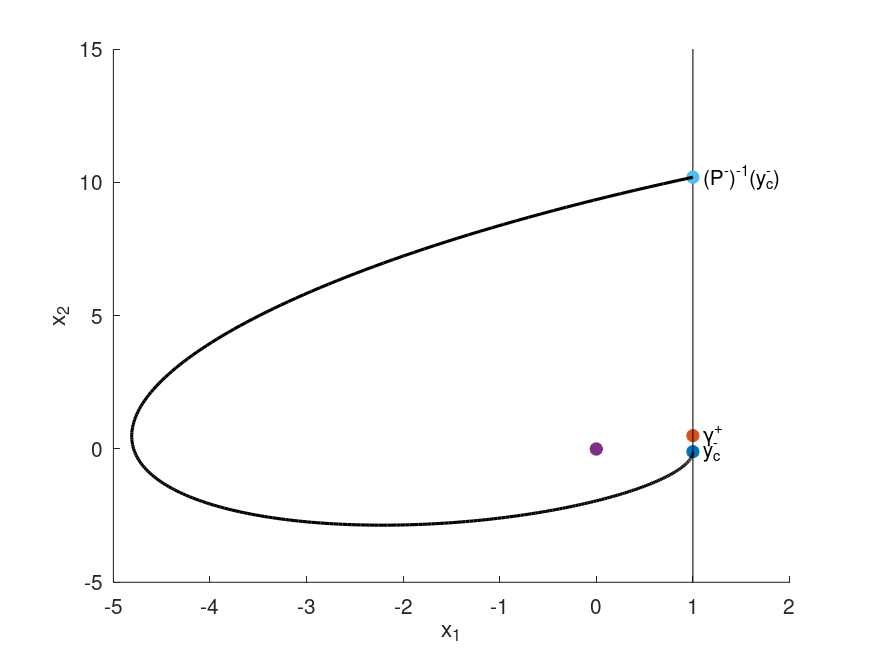
\includegraphics[width=7cm]{aaaaaa}
&
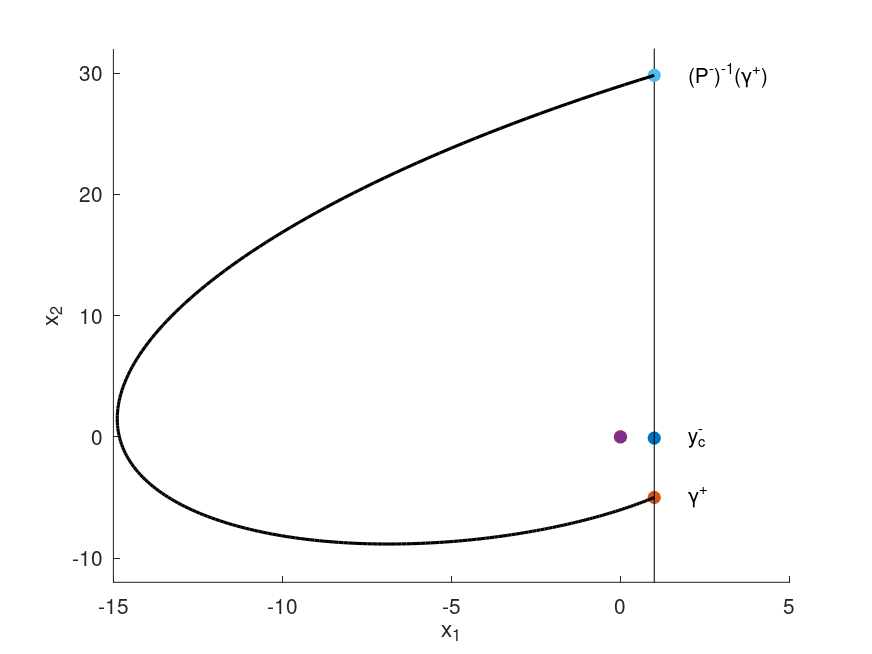
\includegraphics[width=7cm]{dddddd}\\
\small$\gamma^-<0$, $\gamma^+>y_c^-$&\small$\gamma^-<0$, $\gamma^+<y_c^-$\\
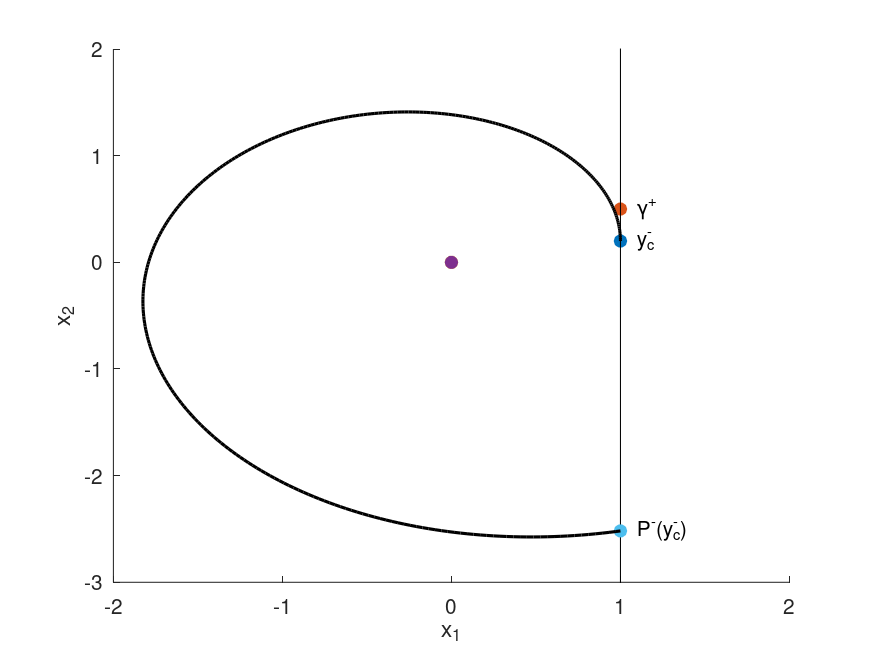
\includegraphics[width=7cm]{cccccc}
&
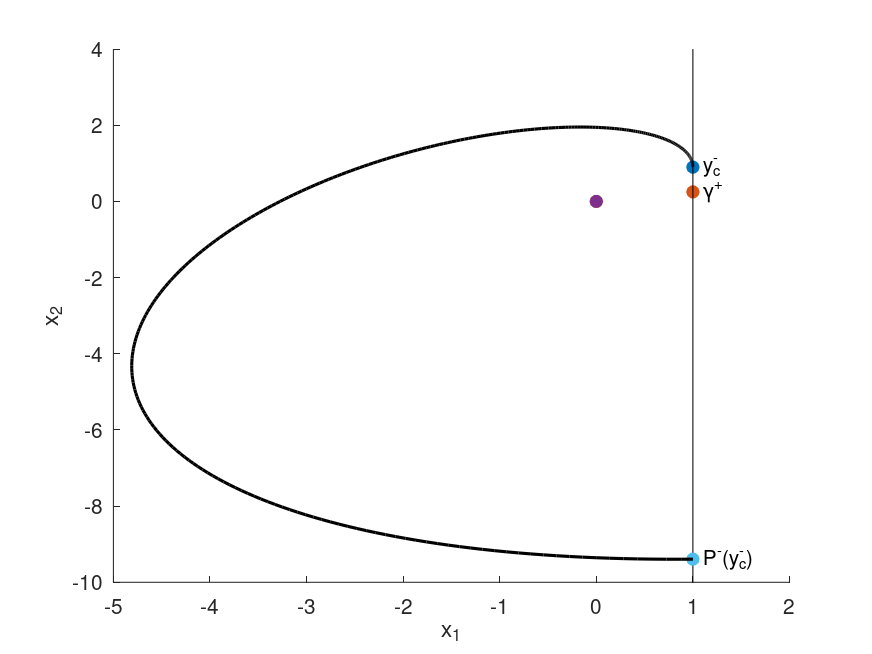
\includegraphics[width=7cm]{bbbbbb}\\
\small$\gamma^->0$, $\gamma^+>y_c^-$&\small$\gamma^->0$, $P^-(y_c^-)<\gamma^+<y_c^-$
\end{tabular}
\end{table}
\begin{figure}[H]
\centering
\begin{table}[H]
\centering
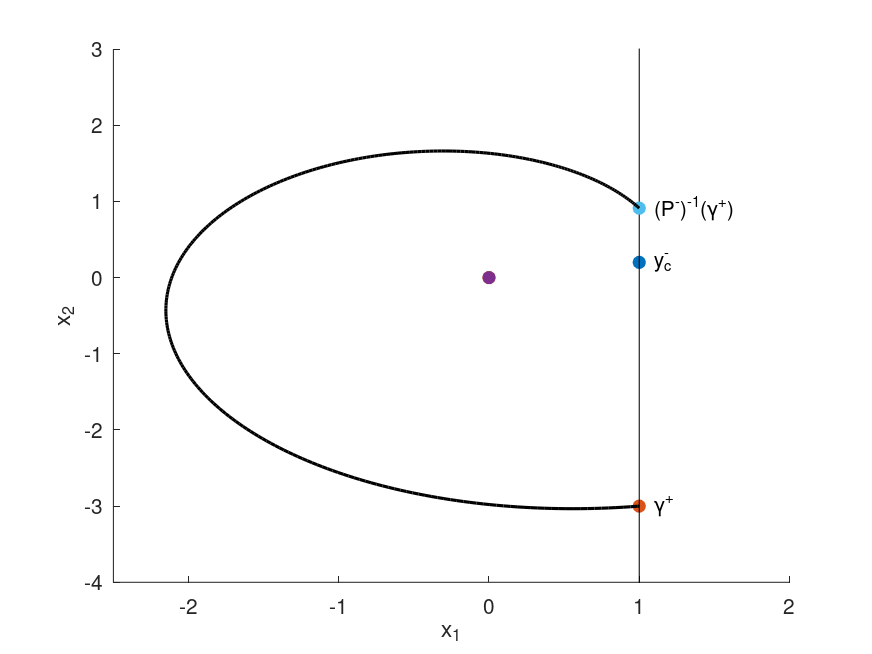
\includegraphics[width=7cm]{eeeeee}\\
\small$\gamma^->0$, $P^-(y_c^-)>\gamma^+$
\end{table}
\caption{\label{mincicle}Menor órbita em casos significativos.}
\end{figure}

O mapa de retorno de Poincaré de (\ref{eqn:jor}) pode finalmente ser definido como
\begin{equation}
\label{eqn:poinc}
P=P^+\circ P^-: y_0\mapsto y_2\text{,  }y_0\in[y_*^-, \infty).
\end{equation}

Um ciclo limite acontece quando $P(y_0)=y_0$ e é definido como uma órbita fechada isolada. De (\ref{eqn:poinc}), portanto, é evidente que um ciclo limite ocorre quando $P^-=(P^+)^{-1}$, o que é visualmente discernível como a intersecção das curvas $P^-$ e $(P^+)^{-1}$, fato que será usado mais adiante no estudo de $P$ para auxiliar a visualização. 

Para aliviar a nomenclatura é definido
\begin{equation}
\label{phi}
\varphi_{\gamma}(\tau)=1-\exp (\gamma \tau) (\cos \tau-\gamma \sin \tau),
\end{equation}
e do fluxo $\phi^+$ definido anteriormente é possível definir $y_1$ e $y_2$ de (\ref{right}) em função do tempo de voo entre eles, $\tau^{+}$. Em outras palavras, $\tau^{+}$ é tal que $(1,y_2)^T$ é alcançado sob a ação do fluxo $\phi^+((1,y_1)^T, t)$ após o tempo $\tau^{+}\beta^+$, visualmente representado como o ângulo $(1,y_1)^T\hat{o}(1,y_2)^T$, e que pertence a um intervalo que é graficamente evidente. Logo
\begin{equation}
\label{righttime}
\left\{\begin{array}{l}
y_{1}\left(\tau^{+}\right)=\gamma^{+}-\frac{\exp \left(-\gamma^{+} \tau^{+}\right) \varphi_{\gamma}+\left(\tau^{+}\right)}{\sin \tau^{+}}, \\
y_{2}\left(\tau^{+}\right)=\gamma^{+}+\frac{\exp \left(\gamma^{+} \tau^{+}\right)  \varphi_{-\gamma}+\left(\tau^{+}\right)}{\sin \tau^{+}}
\end{array}, \quad \tau^{+} \in(0, \pi)\right.,
\end{equation}
que possui
$$
y_{2}=-\exp \left(\gamma^{+} \pi\right) y_{1}-\gamma^{+}\left[1+\exp \left(\gamma^{+} \pi\right)\right]
$$
como uma linha assintótica com  $y_{1} \to-\infty$. De forma semelhante, do fluxo $\phi^-$, $y_1$ e $y_2$ de (\ref{left}) são definidos como função do tempo de voo entre eles, $\tau^{-}$. Novamente, $\tau^{-}$ é tal que $(1,y_1)^T$ é alcançado sob a ação do fluxo $\phi^+((1,y_0)^T, t)$ após o tempo $\tau^{-}\beta^-$, visualmente o módulo do ângulo $(1,y_0)^T\hat{o}(1,y_1)^T$, e cujo intervalo ao qual pertence é limitado pela direita pelo tempo de voo da menor órbita, $(1,y_*^-)^T\hat{o}(1,P^-(y_*^-))^T$, denotado $\hat{\tau}^{-}$. Logo
\begin{equation}
\label{lefttime}
\left\{\begin{array}{l}
y_{0}\left(\tau^{-}\right)=\frac{\beta^{-}}{a_{12}^{-}} \cdot \frac{\exp \left(-\gamma^{-} \tau^{-}\right)  \varphi_{\gamma^{-}}\left(\tau^{-}\right)}{\sin \tau^{-}}+y_{c}^{-}, \\
y_{1}\left(\tau^{-}\right)=-\frac{\beta^{-}}{a_{12}^{-}} \cdot \frac{\exp \left(\gamma^{-} \tau^{-}\right)  \varphi_{-\gamma^{-}}\left(\tau^{-}\right)}{\sin \tau^{-}}+y_{c}^{-}
\end{array}\right., \quad \tau^{-} \in\left(\pi, \hat{\tau}^{-}\right),
\end{equation}
que possui
\begin{equation}
\label{assin}
 y_{1}=-\exp \left(\gamma^{-} \pi\right)  y_{0}+\frac{a_{22}^{-}}{a_{12}^{-}} \left[1+\exp \left(\gamma^{-} \pi\right)\right]
\end{equation}
como uma linha assintótica com  $y_{0} \to\infty$. 

Pela análise de (\ref{eqn:poinc}), foram obtidos resultados para o número de ciclos limite no plano $\gamma^+\times \gamma^-$ para $y_c^-=\gamma^+$, enunciados na Proposição 1.
\begin{proposition}
Se $\gamma^{+}=y_{c}^{-}$, as seguintes afirmações são válidas.

(1) Quando $\gamma^{+}=\gamma^{-}=0$, a origem é um centro global do sistema (\ref{eqn:jor}), e existe um contínuo de órbitas periódicas;

(2) Quando $\gamma^{+} \neq 0, \gamma^{-}=0$, a origem é um centro local do sistema (\ref{eqn:jor}), e existe um número infinito de órbitas periódicas;

(3) Quando $\gamma^{+} \cdot \gamma^{-}<0$ e $\left(\gamma^{+}+\gamma^{-}\right) \cdot \gamma^{+}>0$, existe 1 ciclo limite, que é estável se $\gamma^{+}<0$ e instável se $\gamma^{+}>0$;

(4) Quando $\gamma^{+}=0, \gamma^{-} \neq 0$ ou $\gamma^{+} \cdot \gamma^{-}>0$ ou $\gamma^{+} \cdot \gamma^{-}<0,\left(\gamma^{+}+\gamma^{-}\right) \cdot \gamma^{+} \leq 0$, não existem ciclos limite.
\end{proposition}
\textit{Prova.} Veja \cite{Huan:etal:2012}. 

Na Figura \ref{prep1} estão ilustrados alguns exemplos produzidos para essa preposição, com as regiões de atração em torno de um ciclo limite isolado coloridas em azul e as regiões de repulsão em vermelho.
\begin{table}[H]
\centering
\begin{tabular}{cc}
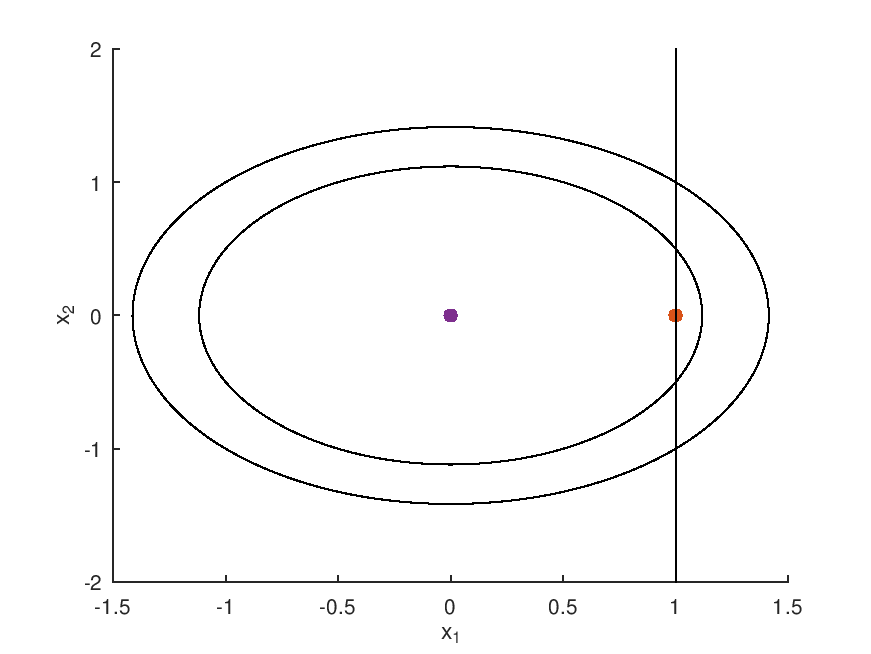
\includegraphics[width=6cm]{1_1}
&
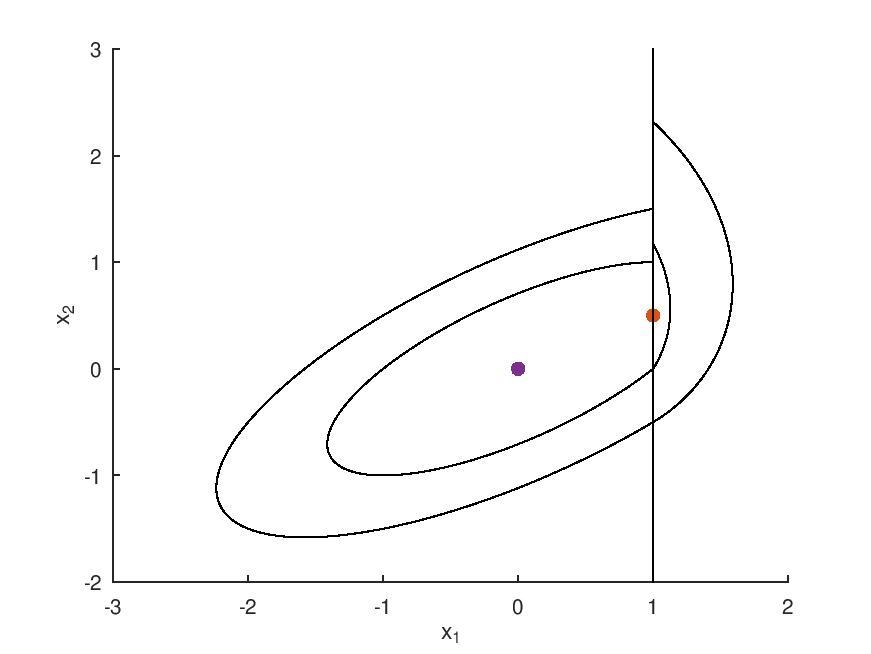
\includegraphics[width=6cm]{1_2}\\
\small(1) $\gamma^+=\gamma^-=0$&\small(2) $\gamma^+\neq0$, $\gamma^-=0$\\
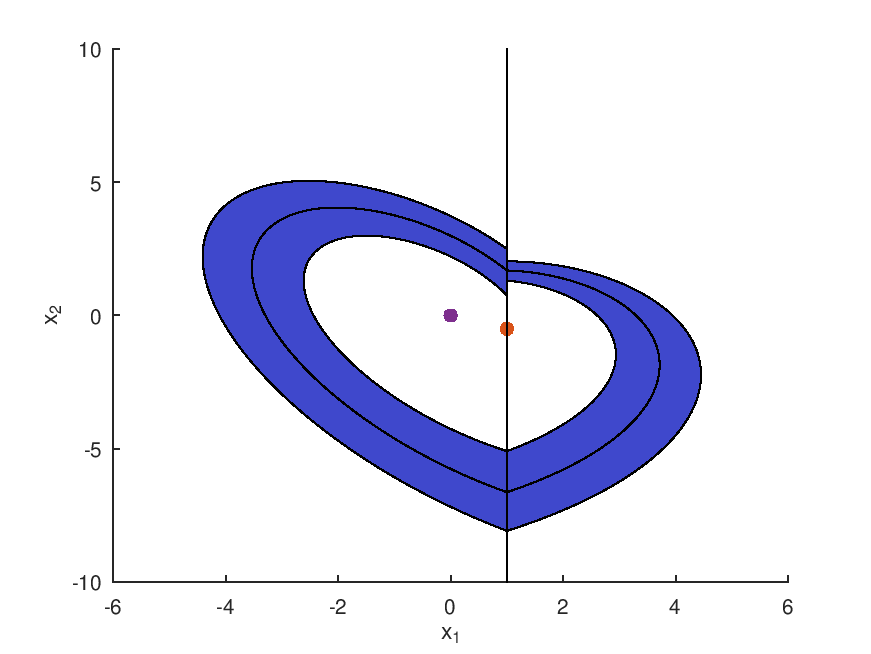
\includegraphics[width=6cm]{1_3_1}
&
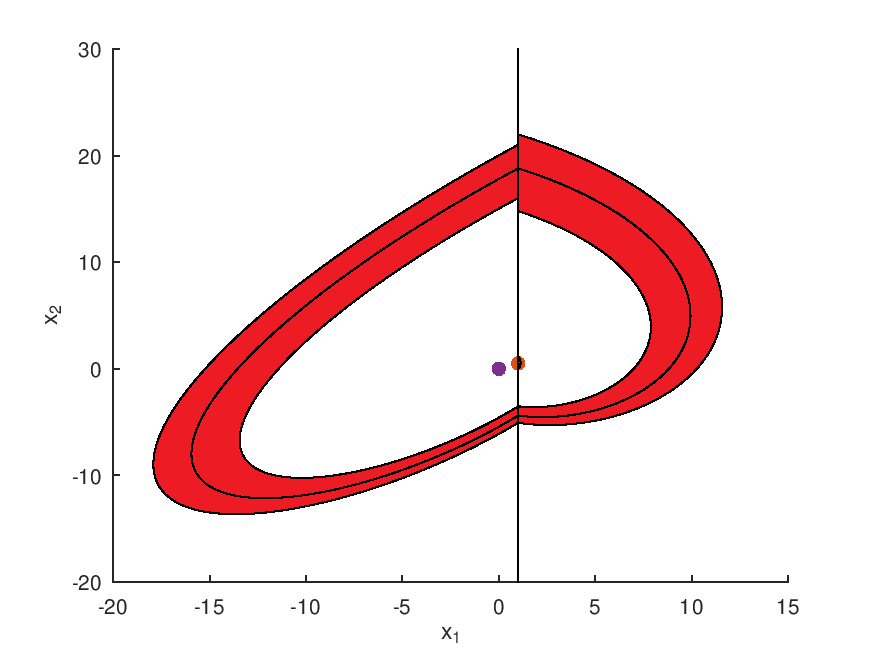
\includegraphics[width=6cm]{1_3_2}\\
\small(3) $\gamma^+\gamma^-<0$, $\gamma^+<0$&\small(3) $\gamma^+\gamma^-<0$, $\gamma^+>0$\\
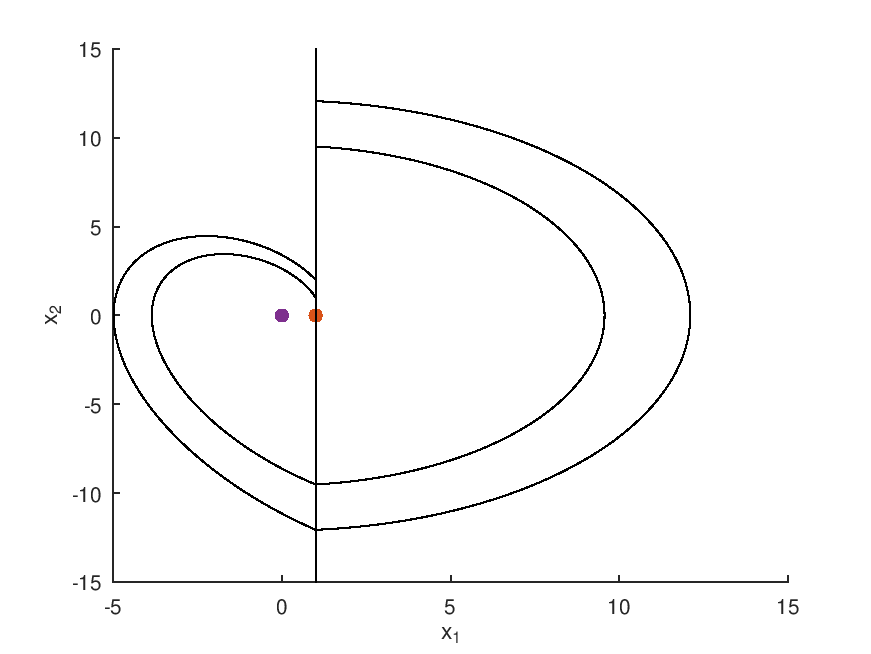
\includegraphics[width=6cm]{1_4_1}
&
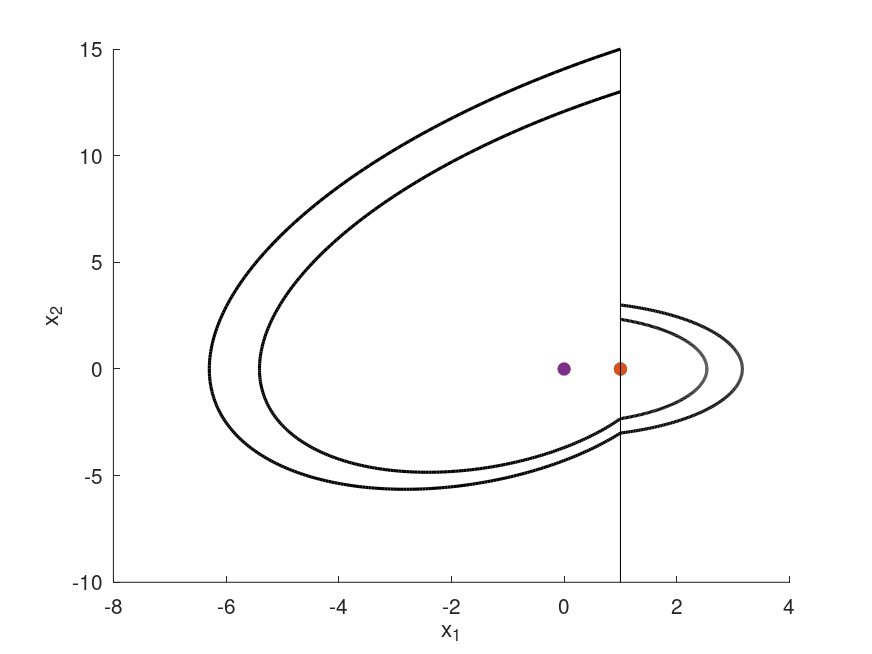
\includegraphics[width=6cm]{1_4_1_lesser}\\
\small(4) $\gamma^+=0$, $\gamma^->0$&\small(4) $\gamma^+=0$, $\gamma^-<0$
\end{tabular}
\end{table}
\begin{figure}[H]
\centering
\begin{table}[H]
\centering
\begin{tabular}{cc}
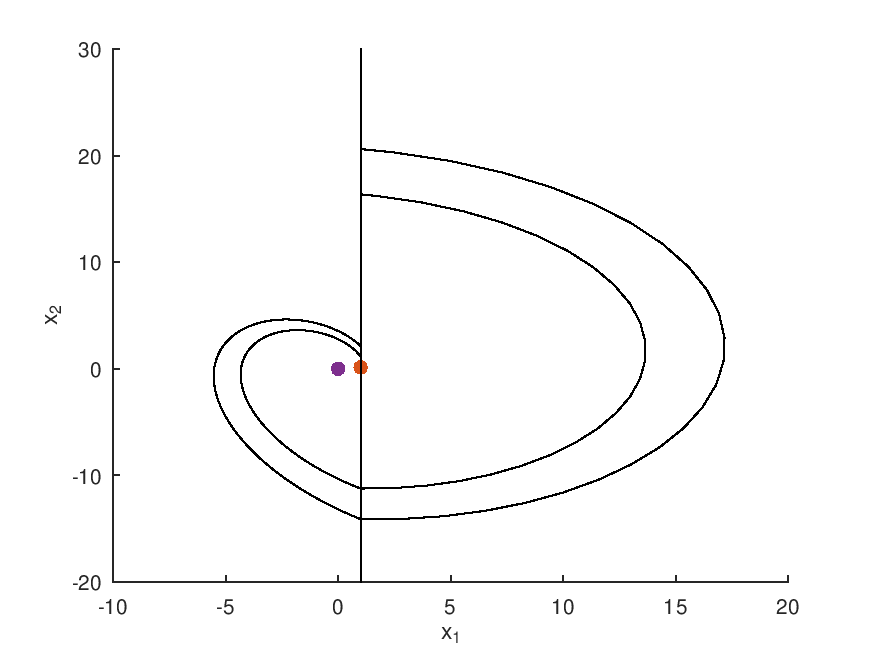
\includegraphics[width=6cm]{1_4_2_greater}
&
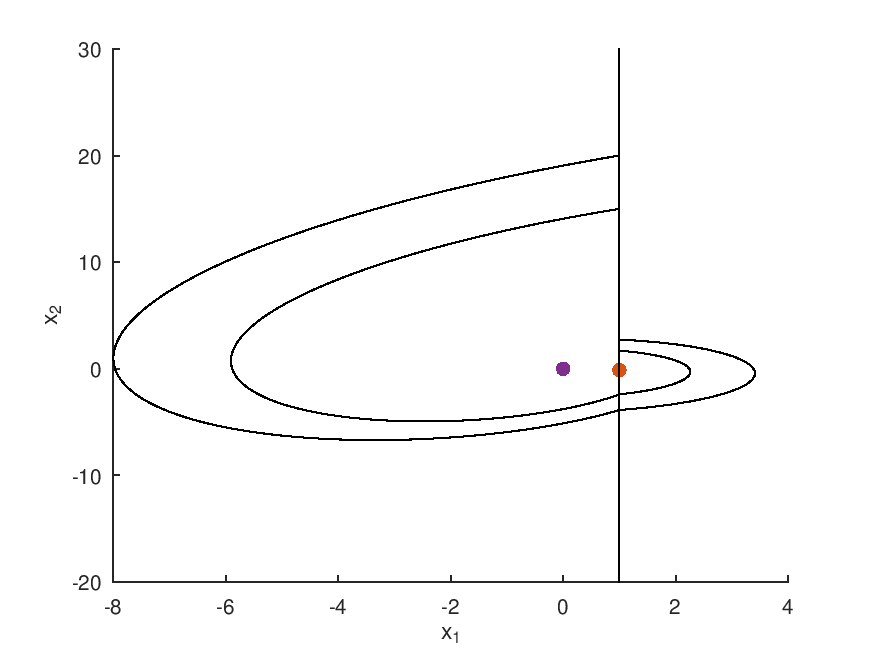
\includegraphics[width=6cm]{1_4_2_lesser}\\
\small(4) $\gamma^+\gamma^->0$, $\gamma^+>0$&\small(4) $\gamma^+\gamma^->0$, $\gamma^+<0$\\
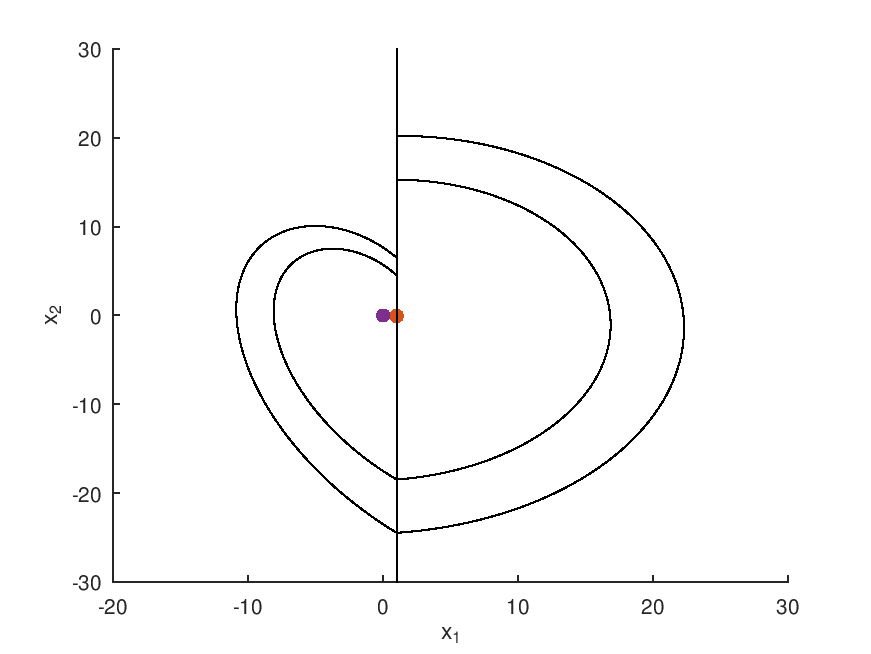
\includegraphics[width=6cm]{1_4_3_plus_negative}
&
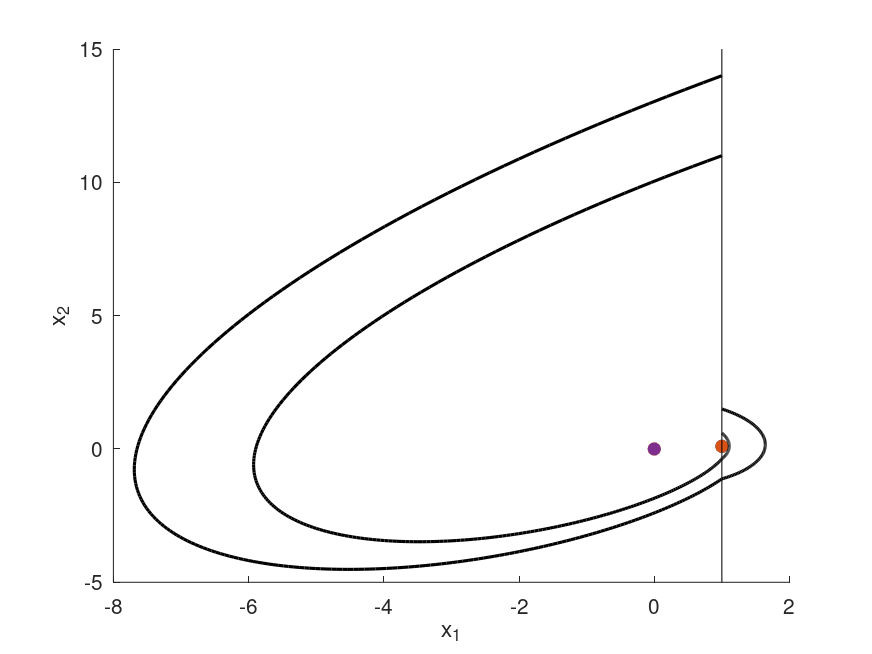
\includegraphics[width=6cm]{1_4_3_plus_positive}\\
\small(4) $\gamma^+\gamma^-<0$, $(\gamma^++\gamma^-)\gamma^+\leq0$, $\gamma^+<0$&\small(4) $\gamma^+\gamma^-<0$, $(\gamma^++\gamma^-)\gamma^+\leq0$, $\gamma^+>0$
\end{tabular}
\end{table}
\caption{\label{prep1}Proposição 1. $\gamma^+=y_c^-$.}
\end{figure}

O caso $y_c^-<\gamma^+$ também já foi abordado, entretanto não no quarto quadrante do plano $\gamma^+\times \gamma^-$ ($\gamma^+>0$, $\gamma^-<0$), que será logo explorado nesse trabalho, e os resultados obtidos são enunciados na Proposição 2.
\begin{proposition}
Se $\gamma^{+}>y_{c}^{-}$, então as seguintes afirmações são válidas.

(1) Quando $\gamma^{+} \geq 0, \gamma^{-} \geq 0$ ou $\gamma^{-} \geq-\gamma^{+}>0$, não existem ciclos limite;

(2) Quando $0 \leq \gamma^{-}<-\gamma^{+}$, existe 1 ciclo limite, que é estável;

(3) Quando $\gamma^{+} \leq 0, \gamma^{-}<0$, existem 0 a 2 ciclos limite. Ademais, para dado qualquer $\gamma^{+}$ e $y_{c}^{-}$, existem duas funções contínuas $f_{12}, f_{21}$, que são decrescentes, tal que

\qquad(a) se $\gamma^{-}>f_{12}\left(\beta^{-} / a_{12}^{-}\right)$, existe 1 ciclo limite, que é estável;

\qquad(b) se $f_{21}\left(\beta^{-} / a_{12}^{-}\right)<\gamma^{-} \leq f_{12}\left(\beta^{-} / a_{12}^{-}\right)$, existem 2 ciclos limite, o maior estável e o menor instável;

\qquad(c) se $\gamma^{-}=f_{21}\left(\beta^{-} / a_{12}^{-}\right)$, existe 1 ciclo limite, que é semi-estável;

\qquad(d) se $\gamma^{-}<f_{21}\left(\beta^{-} / a_{12}^{-}\right)$, não existem ciclos limite.
\end{proposition}
\textit{Prova.} Veja \cite{Huan:etal:2012}.

Na Figura \ref{prep2} estão alguns exemplos produzidos para essa preposição, com a mesma regra de coloração apresentada anteriormente.
\begin{table}[H]
\centering
\begin{tabular}{cc}
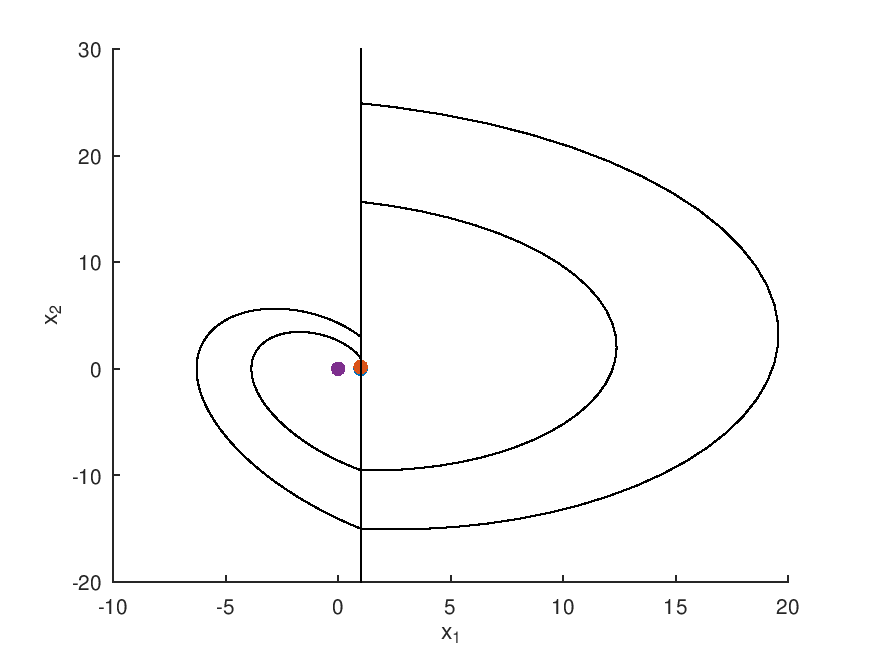
\includegraphics[width=6cm]{2_1_1}
&
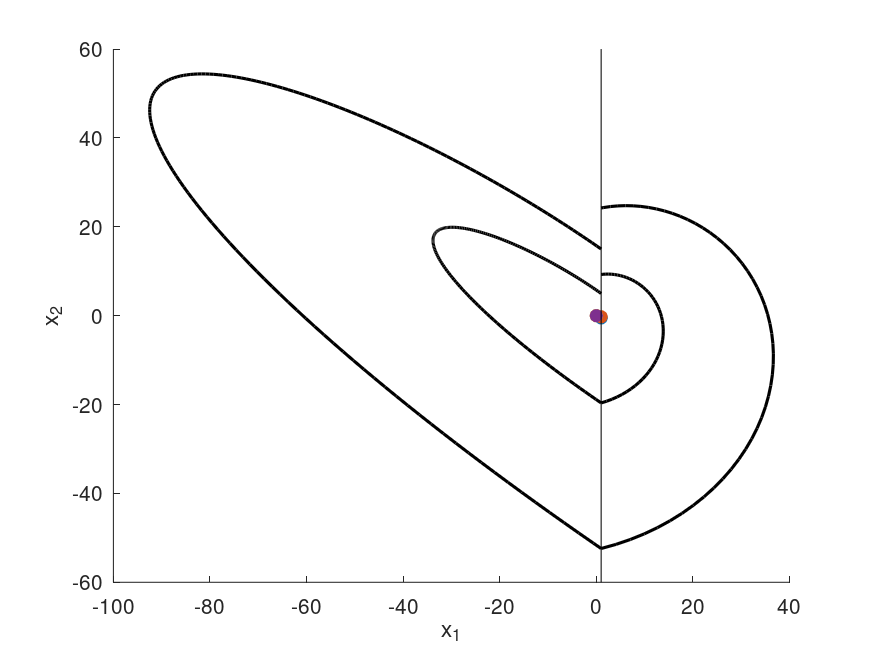
\includegraphics[width=6cm]{2_1_2}\\
\small(1) $\gamma^+\geq0$, $\gamma^-\geq0$&\small(1) $\gamma^-\geq-\gamma^+>0$\\
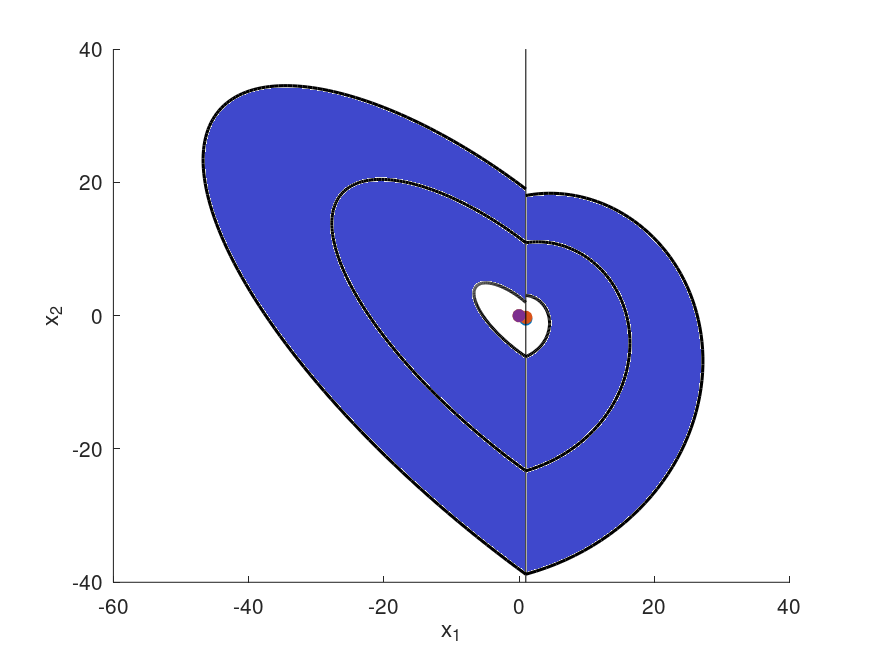
\includegraphics[width=6cm]{2_2}
&
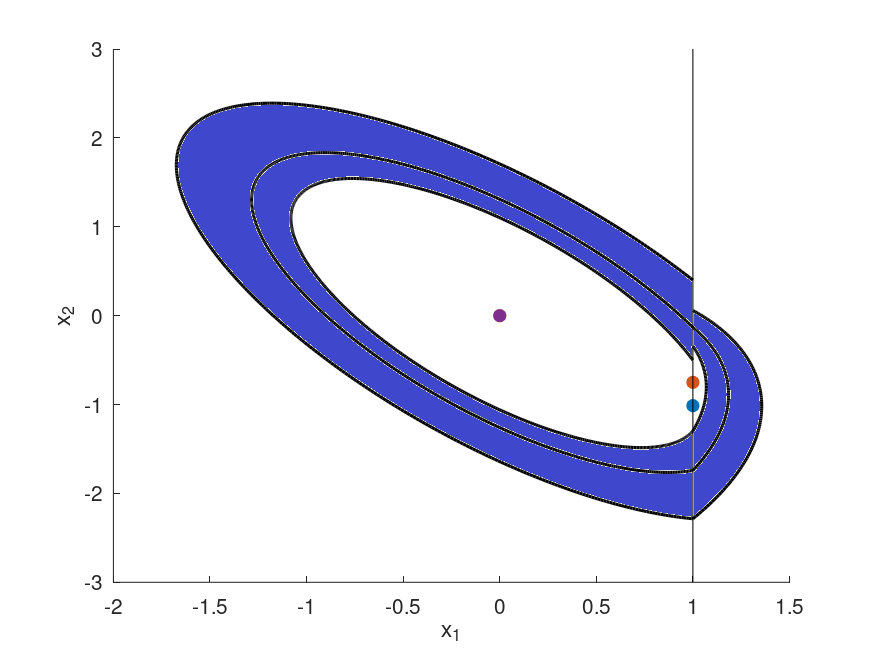
\includegraphics[width=6cm]{2_3_a}\\
\small(2)  $0\leq\gamma^-<-\gamma^+$&\small (3)(a) $\gamma^+\leq0$, $\gamma^-<0$, $\gamma^->f_{12}(\beta^-/a^-_{12})$\\
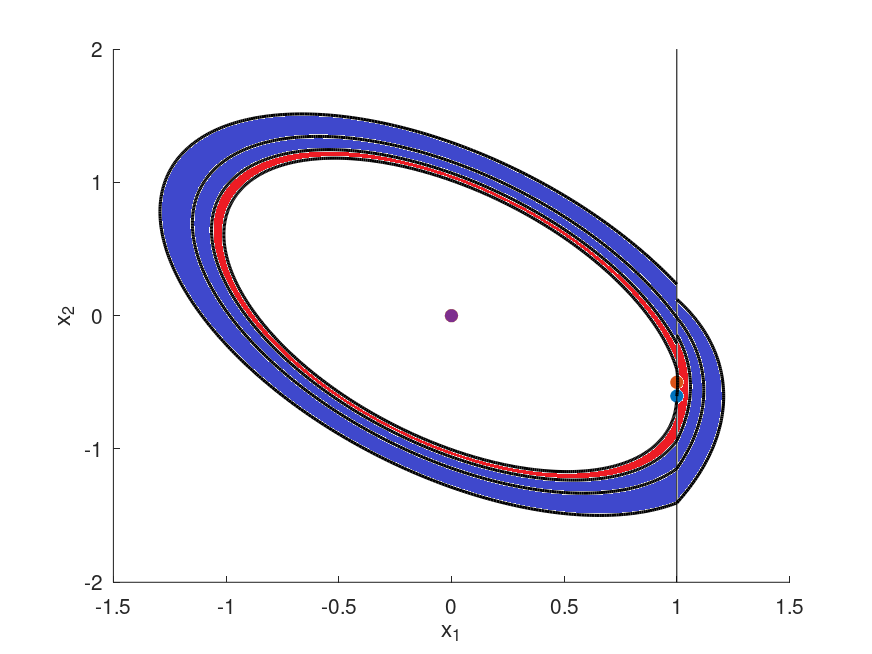
\includegraphics[width=6cm]{2_3_b_eq}
&
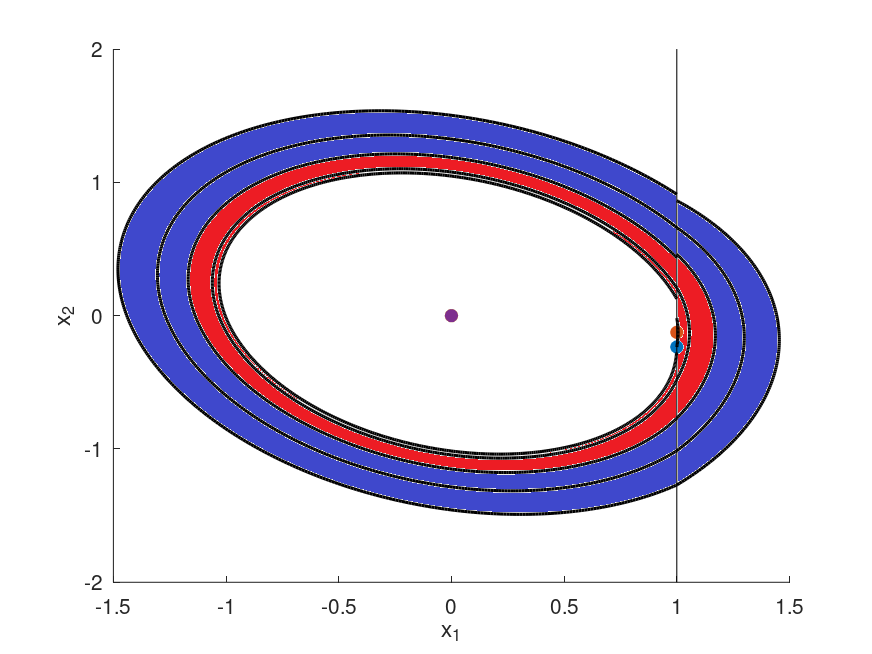
\includegraphics[width=6cm]{2_3_b_less}\\
\small(3)(b) $\gamma^+\leq0$, $\gamma^-<0$, $\gamma^-=f_{12}(\beta^-/a^-_{12})$&\small(3)(b) $\gamma^+\leq0$, $\gamma^-<0$, $f_{21}(\beta^-/a^-_{12})<\gamma^-<f_{12}(\beta^-/a^-_{12})$
\end{tabular}
\end{table}
\begin{figure}[H]
\centering
\begin{table}[H]
\centering
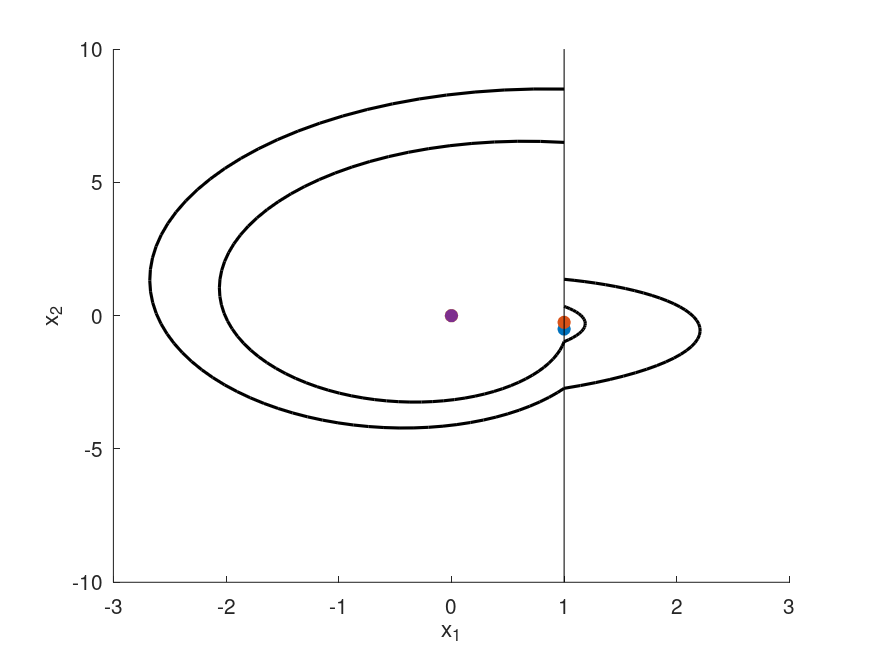
\includegraphics[width=6cm]{2_3_d}\\
\small(3)(d) $\gamma^+\leq0$, $\gamma^-<0$, $\gamma^-<f_{21}(\beta^-/a^-_{12})$
\end{table}
\caption{\label{prep2}Proposição 2.}
\end{figure}
O caso $y_c^->\gamma^+$ (também presente em \cite{Huan:etal:2012}) é de consequência trivial e seus exemplos não apresentam diferenças visuais esclarecedoras em comparação aos da Proposição 2, uma vez que sua prova é baseada na invariabilidade descrita em (\ref{eqn:inva}). 

Para explorar o quarto quadrante do caso $y_c^-<\gamma^+$,$\gamma^+>0$ e $\gamma^-<0$, e consequentemente, pela invariabilidade já citada, o caso $\gamma^+ < y_c^-$, $\gamma^+ < 0$, $\gamma^- > 0$,  	que segundo \cite{Huan:etal:2012} possuem de 0 a 3 ciclos limites, é preciso alguns preparativos. De aqui em diante serão explicados os passos para a obtenção de uma matriz $A^-$ a partir de um $\gamma^+>0$ (e consequentemente uma matriz $J^+$) para que (\ref{eqn:jor}) possua 3 ciclos limites. 

É possível construir uma matriz $A^-$ sob especificação através da relação
\[
A^-=\mathbf{M}^-\mathbf{J}^-(\mathbf{M}^-)^{-1},
\]
onde
\[
\mathbf{J}^{-}=\left(\begin{array}{cc}
\alpha^{-} & -\beta^{-} \\
\beta^{-} & \alpha^{-}
\end{array}\right)
\]
e
\[
\mathbf{M^-}=\left(\begin{array}{cc}
1 & 1 \\
m^-+in^- & m^--in^- 
\end{array}\right),
\]
sendo cada coluna de $\mathbf{M}$, por construção,  os autovalores de $A^-$, e $\alpha^-$ a parte real dos autovalores de $A^-$ e $\beta^-$ a parte imaginária (positiva) dos mesmos. A matriz $A^-$ será da forma
\[
A^-=
\begin{pmatrix}
\alpha^--\frac{m^-\beta^-}{n^-}& \frac{\beta^-}{n^-}\\ 
-\beta^-\left(n^-+\frac{(m^-)^2}{n^-}\right)& \alpha^-+\frac{m^-\beta^-}{n^-}
\end{pmatrix},
\]
e tomando $n^-=\alpha^-$, 
\begin{equation}
\label{amin}
A^-=
\begin{pmatrix}
\alpha^--\frac{m^-}{\gamma^-}& \frac{1}{\gamma^-}\\ 
-\beta^-\left(\alpha^-+\frac{(m^-)^2}{\alpha^-}\right)& \alpha^-+\frac{m^-}{\gamma^-}
\end{pmatrix},
\end{equation}
sendo
\begin{equation}
\label{yc}
y_c^-=-\frac{a^-_{1,1}}{a^-_{1,2}}=m^--\alpha^-\gamma^-.
\end{equation}

Deixando $\beta^-$ e $m^-$ arbitrários fixos, de (\ref{righttime}) e (\ref{lefttime}), para garantir que $y_c^-<\gamma^+$, de (\ref{yc}) tem-se que
\begin{equation}
\label{yc_gammaplus}
(\alpha^-)^2>\frac{m^--\gamma^+}{\beta^-}.
\end{equation}

Além disso, para que $\gamma^-<0$, como $\beta^->0$,
\begin{equation}
\label{alphaneg}
\alpha^-<0.
\end{equation}

Para satisfazer que a menor órbita seja um ciclo limite, ou seja, $P(y^-_*)=y^-_*$, sendo, de (\ref{yast}), $y^-_*=(P^-)^{-1}(y^-_c)$ nesse caso, tem-se que, de (\ref{lefttime}) e (\ref{righttime})
$$
\left\{\begin{array}{l}
y_{c}^{-}=\gamma^{+}-\frac{\exp \left(-\gamma^{+} \hat{\tau}^{+}\right)  \varphi_{\gamma^{+}}\left(\hat{\tau}^{+}\right)}{\sin \left(\hat{\tau}^{+}\right)} \\
\frac{\beta^{-}}{a_{12}^{-}} \cdot \frac{\exp \left(-\gamma^{-} \hat{\tau}^{-}\right)  \varphi_{\gamma^{-}}\left(\hat{\tau}^{-}\right)}{\sin (\hat{\tau}^{-})}+y_{c}^{-}=\gamma^{+}+\frac{\exp \left(\gamma^{+} \hat{\tau}^{+}\right)  \varphi_{-\gamma^{+}}\left(\hat{\tau}^{+}\right)}{\sin \left(\hat{\tau}^{+}\right)}
\end{array}\right.,
$$
sendo $\hat{\tau}^{+}$ o tempo de voo entre $y_c^-$ e  $y^-_*$ para (\ref{right}), isto é, o ângulo $(1,y_c^-)^T\hat{o}(1,y^-_*)^T$. Da relação acima é possível obter uma função erro em função de $\alpha^-$,
\begin{equation}
\label{zero}
f\left( \alpha^-\right)=\frac{1}{\hat{\tau}^-} \log\left(\frac{\sin(\hat{\tau}^-)a^-_{1,2}\left(exp(-\gamma^+\hat{\tau}^+)\varphi_{\gamma^{+}}\left(\hat{\tau}^{+}\right)+exp(\gamma^+\hat{\tau}^+)\varphi_{-\gamma^{+}}\left(\hat{\tau}^{+}\right)\right)}{\sin(\hat{\tau}^+)\beta^-\varphi_{\gamma^{-}}\left(\hat{\tau}^{-}\right)}\right)+\gamma^-,
\end{equation}
onde $\hat{\tau}^\pm$ dependem de $\gamma^-$ e/ou $y_c^-$, logo dependem de $\alpha^-$, por (\ref{yc}) e (\ref{gminus}). Portanto é possível garantir a propriedade da menor órbita ser ciclo limite obtendo-se o zero de tal função erro. Segue, na Figura \ref{igua}, um exemplo de (\ref{eqn:jor}) obtido numericamente satisfazendo tal condição, com
\[
A^-=
\begin{pmatrix}
0.646416386812412& -1\\
1.4225& -0.653583613187589
\end{pmatrix}
\]
e
\[
A^+=
\begin{pmatrix}
0.75& -1\\
1& 0.75
\end{pmatrix}.
\]
\begin{figure}[H]
\centering
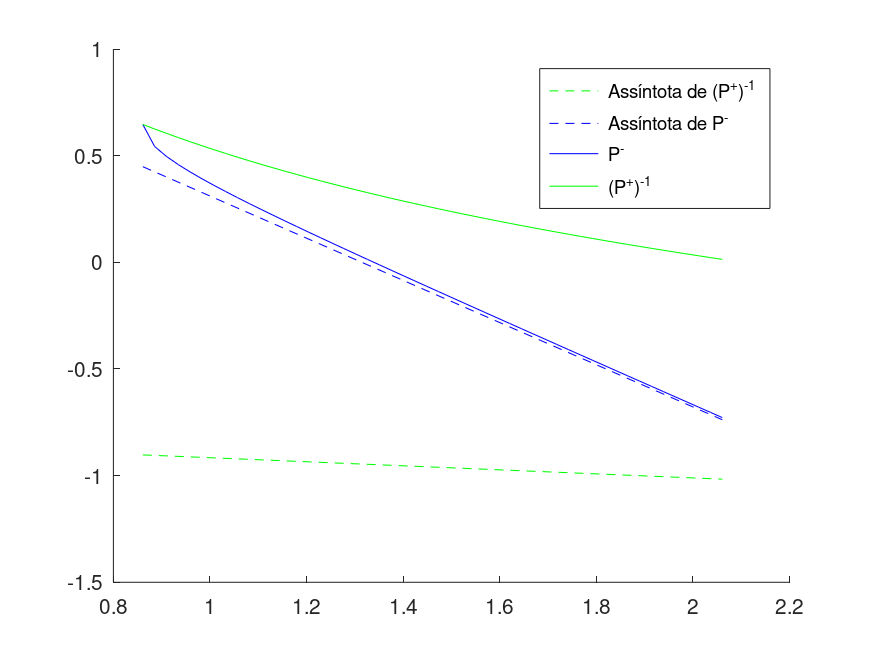
\includegraphics[width=10cm]{poinc}\\
\vspace{\baselineskip}
\caption{\label{igua}Gráfico de $P^-$ e $(P^+)^{-1}$ com $P(y^-_*)=y^-_*$.}
\end{figure}

Além disso, $m^-$ será escolhido de forma que a linha assintótica de (\ref{lefttime}) seja valorada $c<\gamma^+$ em $y^-_*$, isto é, a assíntota passa pelo ponto $C=(y^-_*,c)^T$. De (\ref{amin})
\begin{align*}
\frac{a^-_{2,2}}{a^-_{1,2}}(1+exp(\gamma^-\pi))-exp(\gamma^-\pi)y_*^-&=c \\
\Rightarrow\left(\alpha^-\gamma^-+m^-\right)(1+exp(\gamma^-\pi))-exp(\gamma^-\pi)y_*^-&=c \\
\Rightarrow m^-&=\frac{c+exp(\gamma^-\pi)y_*^-}{1+exp(\gamma^-\pi)}-\gamma^-\alpha^-.
\end{align*}

É possível unir essa condição com a nulidade de (\ref{zero}), isto é, tendo como variável $\alpha^-$, em cada iteração da busca do zero desta última é efetuada uma busca do zero da função erro
\begin{equation}
\label{zero2}
g(m^-)=\frac{c+exp(\gamma^-\pi)y_*^-}{1+exp(\gamma^-\pi)}-\gamma^-\alpha^--m^-,
\end{equation}
onde $y_*^-$ depende de $m^-$ e $\alpha^-$ é fixo. Na Figura \ref{c03} segue um exemplo de (\ref{eqn:jor}) obtido numericamente satisfazendo a nulidade de (\ref{zero}) e (\ref{zero2}) simultaneamente, com a mesma matriz $A^+$ do exemplo da Figura \ref{igua} (de agora em diante não serão expressas as formas de $A^-$, pois estas podem ser obtidas com os parâmetros fornecidos e o algoritmo presente no Apêndice, caso desejado).
\begin{figure}[H]
\centering
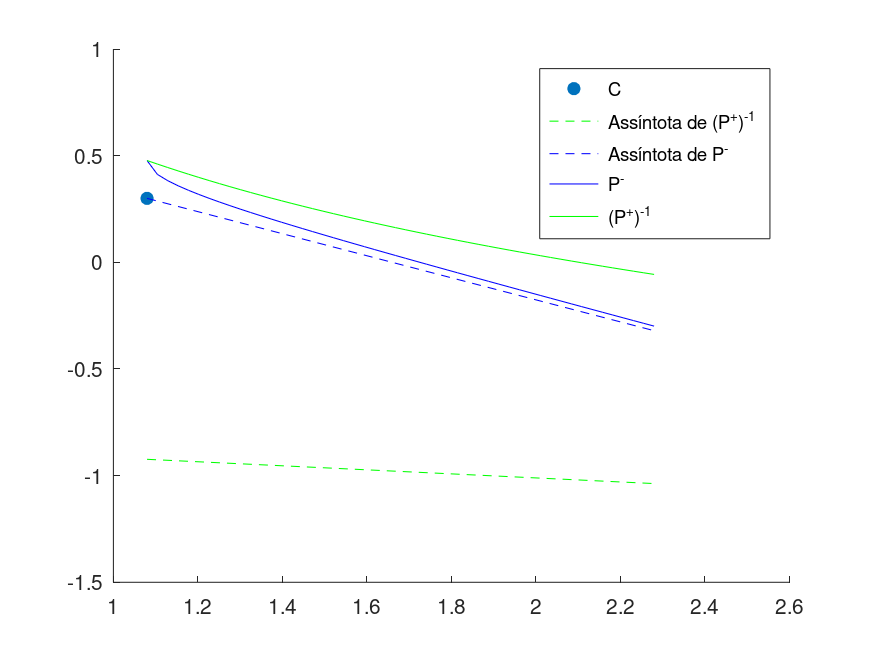
\includegraphics[width=10cm]{poinc3}\\
\vspace{\baselineskip}
\caption{\label{c03}Gráfico de $P^-$ e $(P^+)^{-1}$ com $P(y^-_*)=y^-_*$, $\gamma^+=0.75$, $\beta^-=1$ e $c=0.3$.}
\end{figure}

Dado $\beta^-,\gamma^+>0$ e $c<\gamma^+$ arbitrários e um $m^-(\beta^-,\alpha^-, c)$ satisfazendo a nulidade de (\ref{zero2}), de (\ref{yc_gammaplus}) e (\ref{alphaneg}), $\alpha^-_*$ satisfazendo
\[
(\alpha^-_*)^2=\frac{1}{\beta^-}\cdot\left(\frac{c+exp(\gamma^-\pi)y_*^-}{1+exp(\gamma^-\pi)}-\gamma^-\alpha^-_*-\gamma^+\right),\text{ }\alpha^-_*<0
\]
é o limitante inferior de $\alpha^-$, isto é, $y_c^-(\alpha^-_*)=\gamma^+$. Além disso, de (\ref{yc}) e (\ref{zero2}), com $\alpha^-\to 0^-$ tem-se que $m^-, y_c^-\rightarrow c<\gamma^+$. De (\ref{zero}) e (\ref{phi}), $\lim_{\alpha^-\to 0^-} f(\alpha^-)=\infty$, e $\lim_{\alpha^-\to (\alpha^-_*)^+} f(\alpha^-)=-\infty$, uma vez que $\lim_{\alpha^-\to (\alpha^-_*)^+}\hat{\tau}^+= 0$ da definição de $\hat{\tau}^+$. Logo existe $\alpha^-(\beta^-, c)\in(\alpha^-_*,0)$ tq. $f(\alpha^-)=0$, como pode ser visto na Figura \ref{curve}.
\begin{figure}[H]
\centering
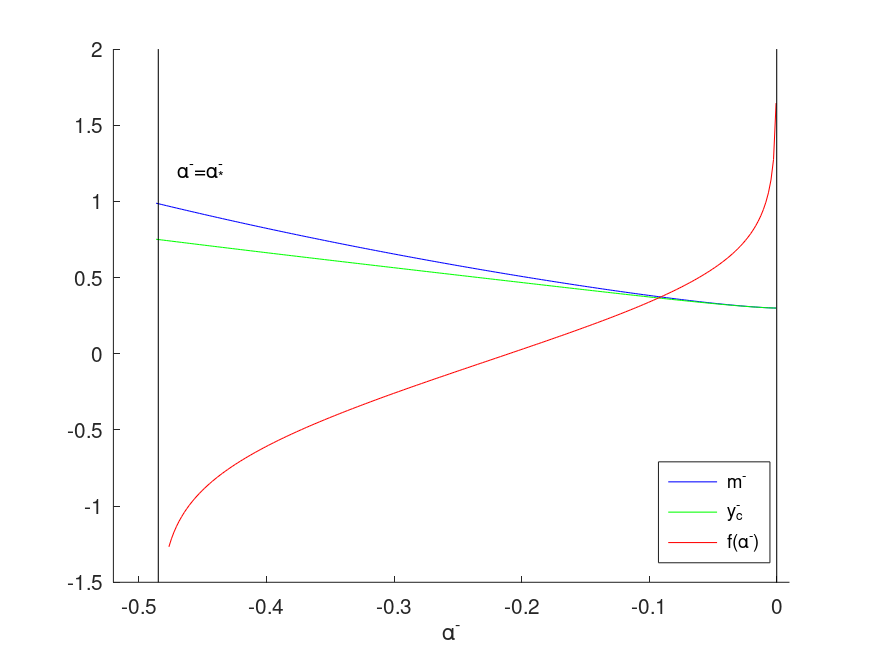
\includegraphics[width=10cm]{curve}\\
\vspace{\baselineskip}
\caption{\label{curve}Gráfico de $m^-$, $y_c^-$ e $f(\alpha^-)$ com $\gamma^+=0.75$, $\beta^-=1$ e $c=0.3$.}
\end{figure}

De (\ref{assin}), é possível notar que $\beta^-$ afeta a inclinação da assíntota de $P^-$ (e consequentemente o comportamento de $P$). Pautando-se no exemplo da Figura \ref{c03}, a Figura \ref{beta1} mostra um exemplo de (\ref{eqn:jor}) que ilustra o efeito da variação de $\beta^-$. 
\begin{figure}[H]
\centering
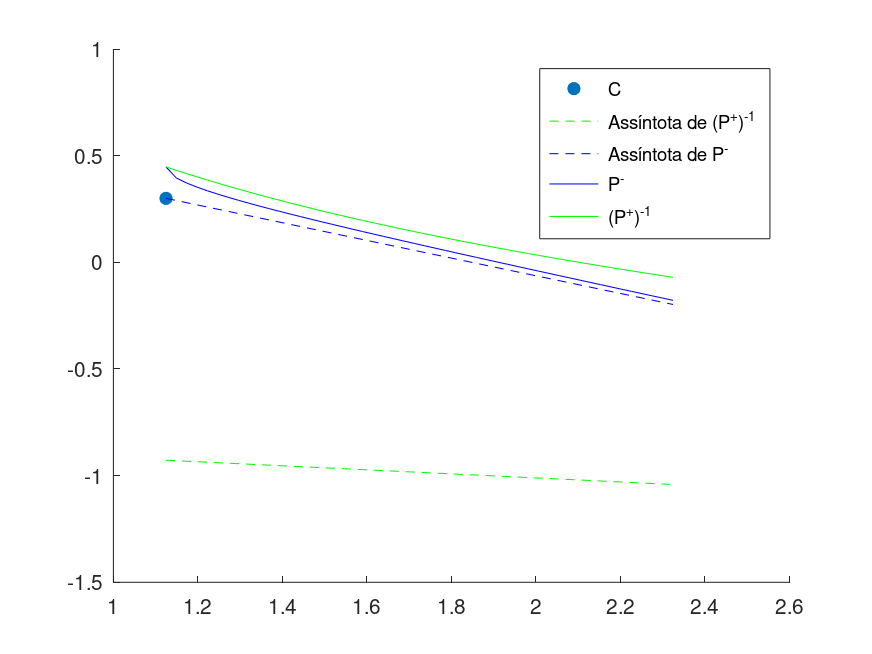
\includegraphics[width=10cm]{poinc2}\\
\vspace{\baselineskip}
\caption{\label{beta1}Gráfico de $P^-$ e $(P^+)^{-1}$ com $P(y^-_*)=y^-_*$, $\gamma^+=0.75$, $\beta^-=0.6$ e $c=0.3$.}
\end{figure}

Outra variável que pode ser inserida é uma folga $p$ em (\ref{zero}), de forma que ao se zerar a função ajustada com a folga, $P(y^-_*)\neq y^-_*$, porém de forma controlada. Para tal é criada a a função erro ajustada
\begin{equation}
\label{zero3}
f'\left( \alpha^-\right)=f\left( \alpha^-\right)+p,
\end{equation}
cujo efeito ao ser usada no lugar de $f\left( \alpha^-\right)$ pode ser observado na Figura \ref{folga}.
\begin{figure}[H]
\centering
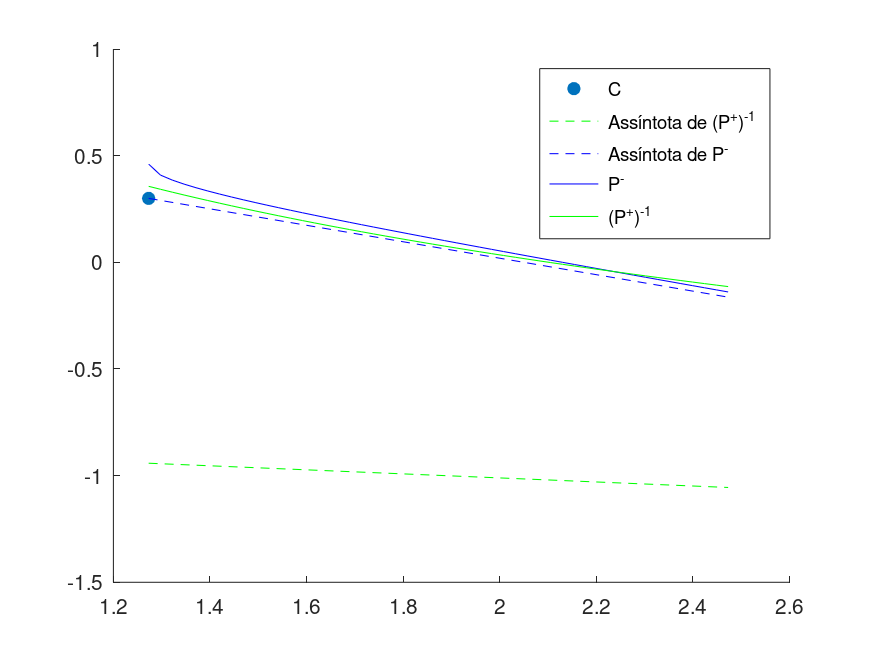
\includegraphics[width=10cm]{folga}\\
\vspace{\baselineskip}
\caption{\label{folga}Gráfico de $P^-$ e $(P^+)^{-1}$ com $f'\left( \alpha^-\right)=0$, $p=0.05$, $\gamma^+=0.75$, $\beta^-=0.6$ e $ c=0.3$.}
\end{figure}
Através das ideias apresentadas, pela forma das curvas de $P^-$ e $(P^+)^{-1}$, conjectura-se que dado um $\gamma^+>0$ qualquer, existe $ \beta^-(\gamma^+)>0$, $c(\gamma^+, \beta^-)<\gamma^+$ e $p(c, \gamma^+, \beta^-)$ tal que 3 ciclos limites se formam (com um exemplo fornecido na Seção 3), ou seja, que as curvas $P^-$ e $(P^+)^{-1}$ se intersectem 3 vezes. Contudo, estudos mais aprofundados do mapa de retorno $P$ ainda precisem ser efetuados para uma conclusão concreta.

\section{Bifurcação de Hopf}
Segundo \cite{Kuznetsov:1998}, uma bifurcação é o fenômeno de surgimento de um retrato de fase topologicamente não equivalente conforme um ou mais parâmetros passam por um valor crítico. Apesar de existirem diversas classificações, aqui será comentado um pouco sobre a bifurcação de Hopf. Esse tipo de bifurcação leva um foco atrator ou repulsor a um estado de atração ou repulsão fraca (não linear), respectivamente, quando os parâmetros atingem o valor crítico, e então para um foco do tipo oposto para valores dos parâmetros após tal ponto crítico. Além disso é formado um ciclo limite em torno do foco em um dos lados do ponto crítico, cuja estabilidade depende do tipo de foco que é englobado; estável (bifurcação supercrítica) para um foco repulsor e instável (bifurcação subcrítica) para um atrator. 

A distinção entre bifurcação subcrítica e supercrítica pode ser entendida com quão~"abruptamente"~uma solução escapa do equilíbrio na sua forma atratora quando o parâmetro é lentamente variado na direção da região na qual o foco passa a ser repulsor, o que é importante para entender se a solução permanecerá em uma vizinhança do equilíbrio de forma não catastrófica ou se será~"ejetada"~catastroficamente, o que é de consideração para o estudo da performance de máquinas sob desgaste ou outras variações externas (que representam a lenta variação dos parâmetros) quando estes atingem um ponto crítico. Para ilustrar essas ideias será apresentado um exemplo dentro do tema de sistemas lineares planares por partes.

Em \cite{HAN20102399} foi estudado o problema auxiliar
\begin{equation}
\label{eqn:hop}
\dot{\mathbf{x}}=\left\{\begin{array}{ll}
\mathbf{A}^{+}\mathbf{x}+b^+  & \text { se } x \geq 0 \\
\mathbf{A}^{-}\mathbf{x}+b^-  & \text { se } x<0
\end{array}
\text{, }\mathbf{x}=
\begin{pmatrix}
x\\
y
\end{pmatrix}
\right.,
\end{equation}
com enfoque no fenômeno de bifurcação. Nele foi provado o seguinte teorema.
\begin{theorem} Dado (\ref{eqn:hop}) com $b^\pm=\vec{0}$ e um foco elementar de tipo FF (focus-focus, isto é, um foco de ambos os  subsistemas) e ordem 1 na origem, sendo $\alpha^\pm$ e $\beta^\pm$ definidos como previamente e
\[
\alpha^+<0,\text{ } \frac{\alpha^+}{\beta^+}+\frac{\alpha^-}{\beta^-} < 0,
\]
então existe uma constante $\varepsilon_{0}>0$ e funções $C^{\infty}$
$$
\begin{gathered}
\varphi_{1}\left(b_{1}^{+}\right)=\frac{\beta^{-}}{\beta^{+}} b_{1}^{+}+O\left(\left|b_{1}^{+}\right|^{2}\right), \text{ } \varphi_{2}\left(b_{1}^{+}\right)=\frac{\alpha^{-}}{\beta^{+}} b_{1}^{+}+O\left(\left|b_{1}^{+}\right|^{2}\right) \\
\varphi_{3}\left(b_{1}^{+}\right)=\frac{\alpha^{+}}{\beta^{+}} b_{1}^{+}+O\left(\left|b_{1}^{+}\right|^{2}\right), \text{ } \tilde{\varphi}\left(b_{1}^{+}, b_{2}^{+}\right)=\frac{\alpha^{-}}{\alpha^{+}} b_{2}^{+}+O\left(\left|b_{1}^{+}, b_{2}^{+}\right|^{2}\right)
\end{gathered}
$$
tal que para $\left|b_{1}^{\pm}\right|+\left|b_{2}^{\pm}\right|<\varepsilon_{0}$, se
$$
b_{2}^{+}<\varphi_{3}\left(b_{1}^{+}\right),\text{ }  \varphi_{2}\left(b_{1}^{+}\right)<b_{2}^{-}<\tilde{\varphi}\left(b_{1}^{+}, b_{2}^{+}\right)
$$
o sistema (\ref{eqn:hop}) possui 1 ciclo limite se $0<\varphi_{1}\left(b_{1}^{+}\right)-b_{1}^{-}\ll 1$ e 2 se $0<b_{1}^{-}-\varphi_{1}\left(b_{1}^{+}\right) \ll 1$.
\end{theorem}
\textit{Prova.} Veja \cite{HAN20102399}.

Tomando 
\[
A^-=\begin{pmatrix}
1&4\\
-1&1
\end{pmatrix},
\]
\[
A^+=\begin{pmatrix}
-1&2\\
-1&-1
\end{pmatrix}
\]
e 
\[
b^\pm=\begin{pmatrix}
0\\0
\end{pmatrix},
\]
a Figura \ref{undist} apresenta o retrato de fase de (\ref{eqn:hop}), no qual a origem é um foco repulsor (repare que o fluxo do sistema é no sentido horário).
\begin{figure}[H]
\centering
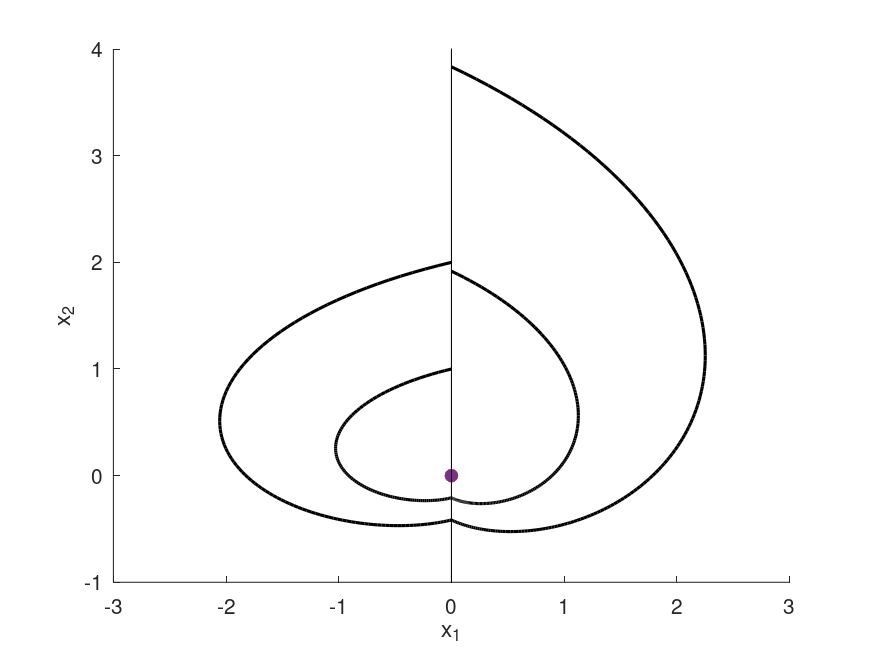
\includegraphics[width=10cm]{disturb_pre}\\
\caption{\label{undist}$b^\pm=\vec{0}$}
\end{figure}
 
Tomando agora o mesmo exemplo, porém com
\[
b^-=\begin{pmatrix}
-0.14\\
0
\end{pmatrix}
\]
e
\[
b^-=\begin{pmatrix}
-0.1\\
-0.1
\end{pmatrix},
\]
é produzido o retrato de fase da Figura \ref{hdist}, na qual o ponto crítico dos parâmetros foi ultrapassado para o caso com $0<\varphi_{1}\left(b_{1}^{+}\right)-b_{1}^{-}\ll 1$, e a origem deixa de ser um foco, entretanto dá-se origem a um ciclo limite atrator em torno dela; apesar de não descrever precisamente uma bifurcação de Hopf, essa transição é análoga e pode ser caracterizada como supercrítica, uma vez que um foco atrator é substituído por dois pontos elementares~"repulsores"~cercados de um ciclo limite estável (região ao seu redor em vermelho), e a solução ao escapar do equilíbrio perde estabilidade de forma não catastrófica (suave), permanecendo em uma vizinhança limitada da origem. O caso subcrítico seria o oposto, no qual dois pontos elementares~"atratores"~cercados por um ciclo limite instável são substituídos por um foco repulsor sem um ciclo limite o cercando, e a solução escapa em uma catastrófica (abrupta) perda de estabilidade.
\begin{figure}[H]
\centering
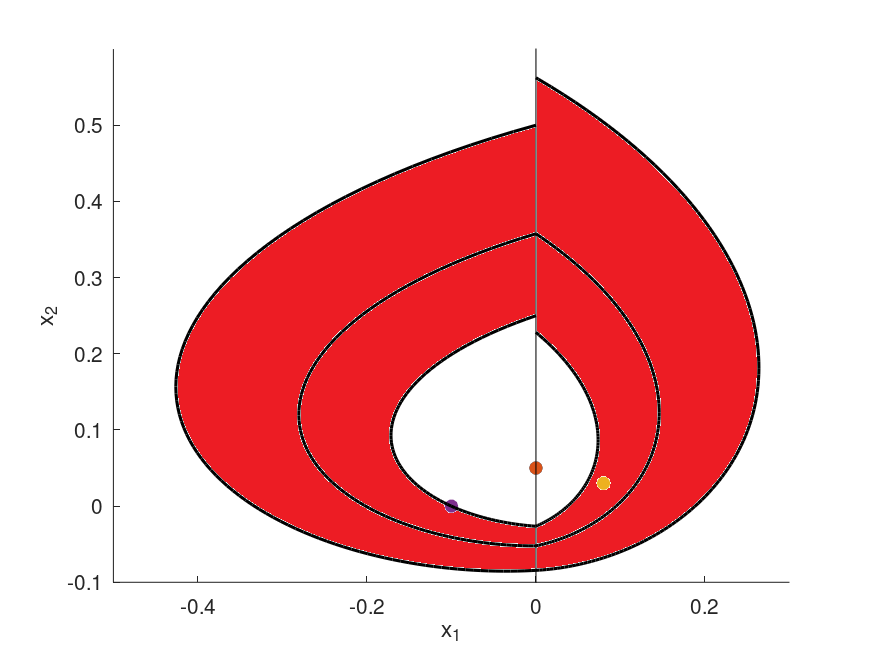
\includegraphics[width=10cm]{disturb_mid}\\
\caption{\label{hdist}$\left|b_{1}^{\pm}\right|+\left|b_{2}^{\pm}\right|<\varepsilon_{0},\text{ }0<\varphi_{1}\left(b_{1}^{+}\right)-b_{1}^{-} \ll 1,\text{ }b_{2}^{+}<\varphi_{3}\left(b_{1}^{+}\right),\text{ }  \varphi_{2}\left(b_{1}^{+}\right)<b_{2}^{-}<\tilde{\varphi}\left(b_{1}^{+}, b_{2}^{+}\right).$}
\end{figure}

Por fim, tomando agora 
\[
b^-=\begin{pmatrix}
-0.14\\
0
\end{pmatrix}
\]
e
\[
b^-=\begin{pmatrix}
-0.1\\
-0.1
\end{pmatrix},
\]
obtém-se o retrato de fase da Figura \ref{dist}, no qual outro ponto crítico foi ultrapassado com o cumprimento de $0<b_{1}^{-}-\varphi_{1}\left(b_{1}^{+}\right) \ll 1$, e um novo ciclo limite se forma entre o anterior e o ponto elementar, desta vez repulsor (região ao seu redor em azul).
\begin{figure}[H]
\centering
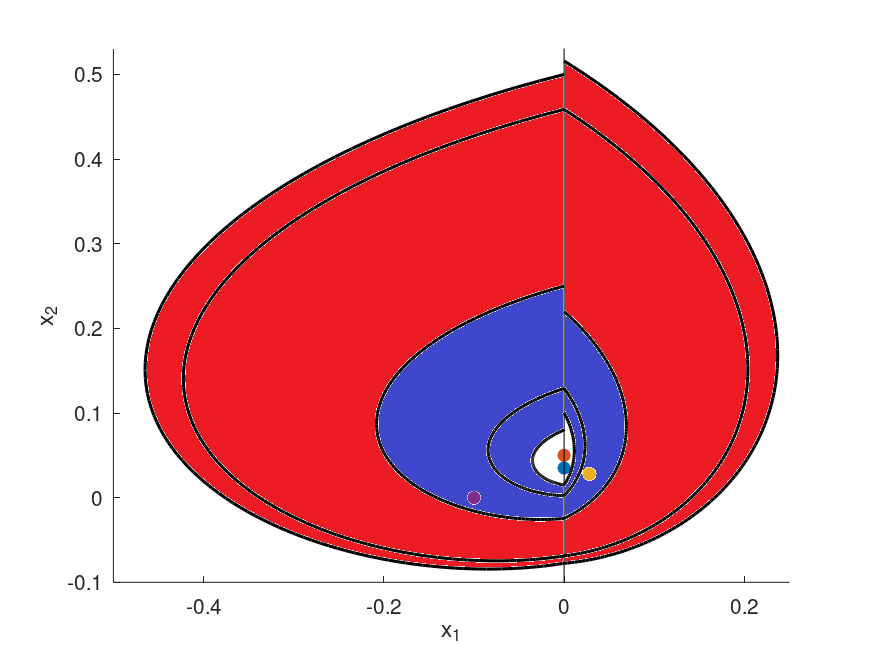
\includegraphics[width=10cm]{disturb_pos}\\
\caption{\label{dist}$\left|b_{1}^{\pm}\right|+\left|b_{2}^{\pm}\right|<\varepsilon_{0},\text{ }0<b_{1}^{-}-\varphi_{1}\left(b_{1}^{+}\right) \ll 1,\text{ }b_{2}^{+}<\varphi_{3}\left(b_{1}^{+}\right),\text{ }  \varphi_{2}\left(b_{1}^{+}\right)<b_{2}^{-}<\tilde{\varphi}\left(b_{1}^{+}, b_{2}^{+}\right).$}
\end{figure}
\section{Resultados}
Utilizando o método descrito na Seção 2.1, dado $\gamma^+$ inicial fixo e variando os parâmetros $ \beta^-$, $c$ e $p$, foi obtido um sistema na forma (\ref{eqn:jor}) que possui 3 ciclos limites, com
\[
A^+=
\begin{pmatrix}
\frac{3}{4}& -1\\
1& \frac{3}{4}
\end{pmatrix}
\]
a forma de Jordan normalizada em $\beta^-$ do subsistema direito (com $\gamma^+=0.75$) e
\[
A^-=
\begin{pmatrix}
13.43538491431723& -18.14977774439898\\
10.01439047867205& -13.50150142642550
\end{pmatrix},
\]
e cujas curvas $P^-$ e $(P^+)^{-1}$ podem ser observadas na Figura \ref{three}, assim como seus parâmetros do método.
\begin{figure}[H]
\centering
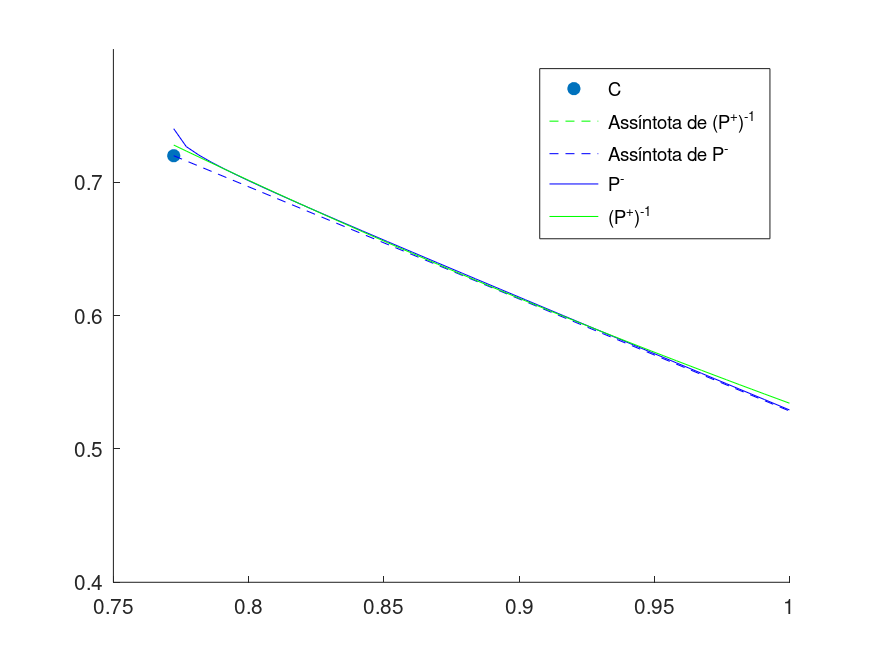
\includegraphics[width=10cm]{three}\\
\vspace{\baselineskip}
\caption{\label{three}Gráfico de $P^-$ e $(P^+)^{-1}$ com $f'\left( \alpha^-\right)=0$, $p=0.09$, $\gamma^+=0.75$, $\beta^-=0.6$ e $ c=0.72$.}
\end{figure}

Uma solução periódica de \ref{eqn:jor} pode ser descrita como a solução $(t^+, t^-, Y)$ do sistema
\begin{align}
\label{u}
&u_{1}\left(t^{+}, t^{-}, Y\right)=x^{+}\left(-t^{+}\right)-1=0 \nonumber\\
&u_{2}\left(t^{+}, t^{-}, Y\right)=x^{-}\left(t^{-}\right)-1=0 \\
&u_{3}\left(t^{+}, t^{-}, Y\right)=y^{+}\left(-t^{+}\right)-y^{-}\left(t^{-}\right)=0\nonumber.
\end{align}

Aqui será provado que o sistema (\ref{u}) das matrizes $A^-$ e $A^+$ apresentadas possui soluções próximas à

\begin{align}
\label{cicl}
&t^+_1 = 0.060050041701417\nonumber,\\
&t^-_1 = 7.536280233527940\nonumber,\\
&Y_1 = 0.791849893551496\nonumber,\\
\nonumber\\
&t^+_2 = 0.090075062552126\nonumber,\\
&t^-_2 = 6.755629691409507,\\
&Y_2 = 0.820743212919858\nonumber,\\
\nonumber\\
&t^+_3 = 0.225187656380317\nonumber,\\
&t^-_3 = 5.899916597164303\nonumber,\\
&Y_3 = 0.928334461670545\nonumber.
\end{align}

Para tal, será usado o método presente em \cite{LilPonce2012}, no qual mais detalhes sobre como achar os limitantes de algumas normas estão presentes, que aqui serão omitidos por brevidade. A base da prova está no seguinte teorema.
\begin{theorem}[Teorema de Newton-Kantorovich]
Dada uma função $u: C \subset \mathbb{R}^{n} \rightarrow \mathbb{R}^{n}$ e $C_{0} \subset C$ convexo, assumindo que $u$ é $\mathcal{C}^{1}$ em $C_{0}$ e que são satisfeitas:

(a) $\left|D u(z)-D u\left(z^{\prime}\right)\right| \leq \gamma\left|z-z^{\prime}\right|$ $\forall z, z^{\prime} \in C_{0}$,

(b) $\left|D u\left(z_{0}\right)^{-1} u\left(z_{0}\right)\right| \leq \alpha$,

(c) $\left|D u\left(z_{0}\right)^{-1}\right| \leq \beta$,
para algum $z_{0} \in C_{0}$. 

Tomando
$$
h=\alpha \beta \gamma, \quad r_{1,2}=\frac{1 \pm \sqrt{1-2 h}}{h} \alpha .
$$

Se $h \leq 1 / 2$ e $\overline{B_{r_{1}}\left(z_{0}\right)} \subset C_{0}$, então a sequência $\left\{z_{k}\right\}$ definida por
$$
z_{k+1}=z_{k}-D u\left(z_{k}\right)^{-1} u\left(z_{k}\right) \text { para } k=0,1, \ldots
$$
é contida em $B_{r_{1}}\left(z_{0}\right)$ e converge ao zero único de $u(z)$ contido em $C_{0} \cap$ $B_{r_{2}}\left(z_{0}\right)$.
\end{theorem}
\textit{Prova.} Veja \cite{Tapia1971}.

Através desse teorema, para cada ponto $(t^+_k, t^−_k, Y_k)$, $k=1, 2, 3$ de (\ref{cicl}), dada as respectivas regiões convexas
$$
\begin{aligned}
&C_{0}^{1}=
[0.06,0.07] \times[7.73,7.54] \times[0.79,0.80],\\
&C_{0}^{2}=[0.09,0.10] \times[6.75,6.76] \times[0.82,0.83],\\
&C_{0}^{3}=[0.22,0.23] \times[5.89,5.90] \times[0.92,0.93]
\end{aligned}
$$
e os respectivos $(\alpha_k, \beta_k, \gamma_k)$
\[
\begin{aligned}
(\alpha_1, \beta_1, \gamma_1)&=(7.3\cdot10^{-8}, 4724,135),
\\
(\alpha_2, \beta_2, \gamma_2)&=(2.4\cdot10^{-8},38647,138),
\\
(\alpha_3, \beta_3, \gamma_3)&=(2\cdot10^{-9},311,142)
\end{aligned}
\]
que satisfazem (a), (b) e (c) do Teorema 1, obtém-se, para cada $k$, respectivamente
\begin{align*}
h^1\approx4.7\cdot10^{-2},\\
h^2\approx1.3\cdot10^{-1},\\
h^3\approx8.8\cdot10^{-5}
\end{align*}
e
\begin{align*}
r_1^1\approx3.1\cdot 10^{-6},\\
r_1^2\approx3.5\cdot10^{-7},\\
r_1^3\approx4.5\cdot10^{-5},    
\end{align*}
que satisfazem as condições finais do teorema ($h^k \leq 1 / 2$ e $\overline{B_{r_{1}^k}\left(z_{0}\right)} \subset C_{0}^k$) e completam a demonstração. Na Figura \ref{triz} os três ciclos limites do sistema podem ser observados.

\begin{figure}[H]
\centering
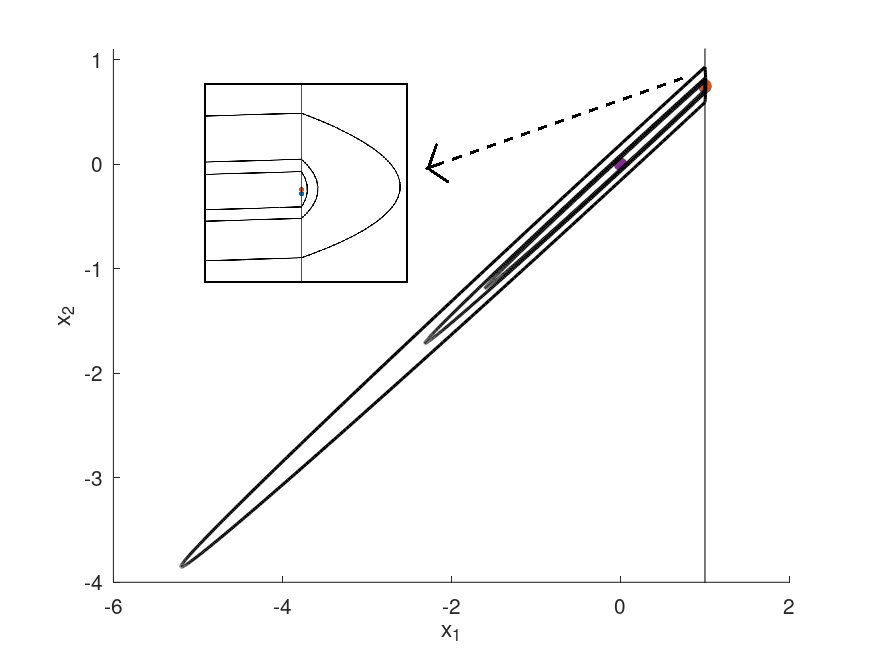
\includegraphics[width=10cm]{triz}\\
\vspace{\baselineskip}
\caption{\label{triz}Três ciclos limite a partir de $\gamma^+=0.75$.}
\end{figure}
\section{Conclusão}
Apesar do sucesso relativo obtido do método de busca de $A^-$ com o caso específico apresentado ($\gamma^+=0.75$), esse foco da pesquisa ainda não está finalizado. Nos próximos meses, pretende-se provar a conjectura de que qualquer $\gamma^+>0$ é candidato do tratamento apresentado para a obtenção de $A^-$ tal que (\ref{eqn:jor}) tenha 3 ciclos limites. Tal análise começará no estudo do mapa de Poincaré nos moldes de \cite{Huan:etal:2012}, utilizando técnicas ali apresentadas para tentar delinear uma demonstração.

Após isso pretende-se estudar o caso de sistemas de equações diferenciais lineares por partes com superfície de descontinuidade $xy=0$, realizando simulações computacionais e obtendo exemplos, com o objetivo
de estabelecer uma conjectura sobre o numero máximo de ciclos limite.
\section{Apêndice}
\begin{lstlisting}[caption={C\'{a}lculo de $P^\pm$ ou $t^\pm$.}, captionpos=b]
function aux=half_poinc(i, Y, t_space, mode, cut, data)
    alpha_minus=real(data{i, 2}(1,1));
    beta_minus=imag(data{i, 2}(1,1));
    if (i==2)
            x=@(t) exp(alpha_minus*t)*(cos(beta_minus*t)*cut-Y*sin(beta_minus*t))-cut;
            y=@(t) exp(alpha_minus*t)*(sin(beta_minus*t)*cut+Y*cos(beta_minus*t));
    else
            m=real(data{i, 1}(2,1));           
            gamma_minus=alpha_minus/beta_minus;
            A_m_diag_dif=-2*m/gamma_minus;
            A_minus_12=1/gamma_minus;
            A_minus_21=-beta_minus*(alpha_minus+m^2/alpha_minus);
            x=@(t) exp(alpha_minus*t)*(cut*(cos(beta_minus*t)+A_m_diag_dif*sin(beta_minus*t)/(2*beta_minus))
            +Y*A_minus_12*sin(beta_minus*t)/beta_minus)-cut;
            y=@(t) exp(alpha_minus*t)*(Y*(cos(beta_minus*t)-A_m_diag_dif*sin(beta_minus*t)/(2*beta_minus))
            +cut*A_minus_21*sin(beta_minus*t)/beta_minus);
    endif
    
    #Busca da inversao
    t_inv=0;
    if (i==1)      
          for t=t_space
              if ((x(t)>0) && (t!=0))
                  t_inv=t;
                  break;
              end
          endfor
    else
          for t=t_space
              if (x(t)<0 && (t!=0))
                  t_inv=t;
                  break;
              end
          endfor
    end
    if (t_inv)
      
        #aux e o t onde a inversao ocorre
        aux=fzero(x, [t_inv-t_space(2), t_inv]);
        Y=y(aux);
    endif
    
    #Retorna Y ao inves de t da inversao
    if (mode)
        aux=Y;
    endif
endfunction
\end{lstlisting}
\begin{lstlisting}[caption={C\'{a}lculo de $\varphi_\gamma(\tau)$.}, captionpos=b]
function phi=calc_phi(tau, gamma)
    phi=1-exp(gamma*tau)*(cos(tau)-gamma*sin(tau));
endfunction
\end{lstlisting}
\begin{lstlisting}[caption={C\'{a}lculo de $g(m^-)$.}, captionpos=b]
function g=calc_g(gamma_minus, alpha_minus, m, beta_minus, cut, data, n_space, t_space, c)
    M=[1, 1; m+alpha_minus*i, m-alpha_minus*i];
    data{1, 1}=M;
    g=(c+exp(gamma_minus*pi)*half_poinc(1, m-alpha_minus*gamma_minus, n_space, 1, cut, data))/(1+exp(gamma_minus*pi))
    -alpha_minus*gamma_minus-m;
endfunction
\end{lstlisting}
\begin{lstlisting}[caption={C\'{a}lculo de $f'(\alpha^-)$.}, captionpos=b]
function f=calc_f(alpha_minus, gamma_plus, data, n_space, t_space, beta_minus, p, cut, c)
    J=[alpha_minus+beta_minus*i, 0; 0, alpha_minus-beta_minus*i];
    gamma_minus=alpha_minus/beta_minus
    data{1, 2}=J;
    m=fzero(@(m) calc_g(gamma_minus, alpha_minus, m, beta_minus, cut, data, n_space, t_space, c), [-100, 100])
    data{1, 1}=[1, 1; m+alpha_minus*i, m-alpha_minus*i];
    scatter(alpha_minus, m, "b");
    
    A_minus=[alpha_minus-m/gamma_minus, 1/gamma_minus; -beta_minus*(alpha_minus+m^2/alpha_minus), alpha_minus+m/gamma_minus];
    
    yc_minus=-A_minus(1, 1)/A_minus(1, 2)
    scatter(alpha_minus, yc_minus, "g");
    
    #yc_minus=-cut*A_minus(1, 1)/A_minus(1, 2);
    tau_plus=half_poinc(2, yc_minus, t_space, 0, cut, data);
    #tau_minus=half_poinc(2, yc_minus, t_space, 0, cut, data)*beta_plus;
    tau_minus=-half_poinc(1, yc_minus, n_space, 0, cut, data)*beta_minus;
    phi_plus_pos=calc_phi(tau_plus, gamma_plus);
    phi_plus_neg=calc_phi(tau_plus, -gamma_plus);
    phi_minus=calc_phi(tau_minus, gamma_minus);
    
    f=log(sin(tau_minus)*A_minus(1,2)*(exp(-gamma_plus*tau_plus)*phi_plus_pos+exp(gamma_plus*tau_plus)*phi_plus_neg)/
    (sin(tau_plus)*beta_minus*phi_minus))/tau_minus+gamma_minus+p
    scatter(alpha_minus, f, "r");
endfunction
\end{lstlisting}
\begin{lstlisting}[caption={Imposi\c{c}\~{a}o de $f'(\alpha^-)=0$ e $g(m^-)=0$ dado $\gamma^+$, $p$, $c$ e $\beta^-$ fixos.}, captionpos=b]
A_plus=[3/4, -1; 1, 3/4];
cut=1;
gamma_plus=-A_plus(1, 1)/A_plus(1, 2);
c=0.72;
beta_minus=0.6;
p=0.09;
#gamma_plus=-cut*A_plus(1, 1)/A_plus(1, 2)

#Se for no sentido horario, colocar t_space decrescente (<=0)
#Mudar o modulo do max t_space e o numero de intervalos se necessario 
#(este ultimo no caso de um sistema passar pelo corte multiplas vezes entre dois passos)
data=cell(2, 2);
t_space=linspace(0, 12, 1200);
n_space=-t_space;

[data{2, 1}, data{2, 2}]=eig(A_plus);

hf=figure;
xlabel("\\alpha^-");
hold on;

alpha_minus=-0.018;
k=0;

#Busca de inversão de f
if (sign(calc_f(alpha_minus, gamma_plus, data, n_space, t_space, beta_minus, p, cut, c))>0)
    do  
        k++
        
        #Passo (alterar se necessario)
        alpha_minus*=1.1
        aux=calc_f(alpha_minus, gamma_plus, data, n_space, t_space, beta_minus, p, cut, c);
        
        #k>n condição de parada secundaria (alterar se necessario)
    until (sign(aux)<0 || k>10)
    start=alpha_minus;
    finish=alpha_minus/1.1;
else
    do
        k++
        
        #Passo (alterar se necessario)
        alpha_minus/=2
        aux=calc_f(alpha_minus, gamma_plus, data, n_space, t_space, beta_minus, p, cut, c);
        
        #k>n condição de parada secundaria (alterar se necessario)
    until (sign(aux)>0 || k>10)
    finish=alpha_minus;
    start=alpha_minus*2;
endif
alpha_minus=fzero(@(alpha_minus) calc_f(alpha_minus, gamma_plus, data, n_space, t_space, beta_minus, p, cut, c),
[start, finish])
legend({"m^-", "y_c^-", "f(\\alpha^-)"}, "location", "southeast");
J=[alpha_minus+beta_minus*i, 0; 0, alpha_minus-beta_minus*i];
gamma_minus=alpha_minus/beta_minus
data{1, 2}=J;
m=fzero(@(m) calc_g(gamma_minus, alpha_minus, m, beta_minus, cut, data, n_space, t_space, c), [0, 100])
A_minus=[alpha_minus-m/gamma_minus, 1/gamma_minus; -beta_minus*(alpha_minus+m^2/alpha_minus), alpha_minus+m/gamma_minus]
text(alpha_minus+0.002, 0.005, "f(\\alpha^-)=0");
hold off;  
\end{lstlisting}
\begin{lstlisting}[caption={C\'{a}lculo de $y_c^-$ e $\gamma^+$ para $b^\pm$ possivelmente n\~{a}o nulo.}, captionpos=b]
function [yc_minus, gamma_plus]=find_elementary(A_minus, A_plus, data, cut)
    yc_minus=-(A_minus(1, 1)*cut+data{1, 4}(1))/A_minus(1, 2);
    gamma_plus=-(A_plus(1, 1)*cut+data{2, 4}(1))/A_plus(1, 2);
endfunction
\end{lstlisting}
\begin{lstlisting}[caption={C\'{a}lculo de $P^\pm$ para $b^\pm$ possivelmente n\~{a}o nulo.}, captionpos=b]
function Y=half_poinc(i, Y, t_space, data, A_minus, cut)
    alpha_minus=real(data{i, 2}(1,1));
    beta_minus=imag(data{i, 2}(1,1));
    d=data{i,3};
    Y_p_x=Y+d(2);
    cut_p_x=cut+d(1);
    if (i==2)
            y=@(t) exp(alpha_minus*t)*(sin(beta_minus*t)*cut_p_x+Y_p_x*cos(beta_minus*t))-d(2);
            x=@(t) exp(alpha_minus*t)*(cos(beta_minus*t)*cut_p_x-Y_p_x*sin(beta_minus*t))-cut_p_x;
    else
            gamma_minus=alpha_minus/beta_minus;
            A_m_diag_dif=A_minus(1,1)-A_minus(2,2);
            x=@(t) exp(alpha_minus*t)*(cut_p_x*(cos(beta_minus*t)+A_m_diag_dif*sin(beta_minus*t)/(2*beta_minus))
            +Y_p_x*A_minus(1,2)*sin(beta_minus*t)/beta_minus)-cut_p_x;
            y=@(t) exp(alpha_minus*t)*(Y_p_x*(cos(beta_minus*t)-A_m_diag_dif*sin(beta_minus*t)/(2*beta_minus))
            +cut_p_x*A_minus(2,1)*sin(beta_minus*t)/beta_minus)-d(2);
    endif
    
    #Busca da inversao
    t_inv=0;
    if (i==1)
          for t=t_space
              if ((x(t)>0) && (t!=0))
                  t_inv=t;
                  break;
              end
          endfor
    else
          for t=t_space
              if (x(t)<0 && (t!=0))
                  t_inv=t;
                  break;
              end
          endfor
    end
    if (t_inv)
      
        #aux e o t onde a inversao ocorre
        aux=fzero(x, [t_inv-t_space(2), t_inv]);
        Y=y(aux);
    endif
endfunction
\end{lstlisting}
\begin{lstlisting}[caption={Fun\c{c}\~{a}o de recurs\~{a}o da busca por ciclos limite de $P$ para $b^\pm$ possivelmente n\~{a}o nulo.}, captionpos=b]
function cycle_at=step_down(start, finish, t_space, data, A_minus, cut)
    h=(finish-start)/2;
    Y=start;
    [start, finish]
    res=[Y, 0];
    cycle_at=[0; 0];
    k=0;
    do
        for i=1:2
            Y=half_poinc(i, Y, t_space, data, A_minus, cut);
        endfor
        si=sign(Y-res(1,1));
        
        #Se houve inversao de comportamento, buscar no subintervalo
        if (res(1,2)*si<0);
            #Caso deseja-se uma precisao maior (menor), diminuir (aumentar) o valor abaixo
            if (h>10^(-9))
                cycle_at=step_down(res(1,1)-h, res(1,1), t_space, data, A_minus, cut);
            else
                cycle_at=[res(1,1)-h; res(1,1)];
            end
            break;
        end
        res=[res(1,1)+h, si];
        Y=res(1,1);
        k++
    until (k==3)
endfunction
\end{lstlisting}
\begin{lstlisting}[caption={Busca por ciclos limite de $P$ para $b^\pm$ possivelmente n\~{a}o nulo.}, captionpos=b]
A_minus=[13.43538491431723,  -18.14977774439898; 10.01439047867205,  -13.50150142642550];
A_plus=[3/4, -1; 1, 3/4];

#Se for no sentido horario, colocar t_space decrescente (<=0)
data=cell(2, 5);
cut=1;

#Mudar o modulo do max t_space e o numero de intervalos se necessario 
#(este ultimo no caso de um sistema passar 
#pelo corte multiplas vezes entre dois passos)
t_space=linspace(0, 18, 1800);
n_space=-t_space;

[data{1, 1}, data{1, 2}]=eig(A_minus);

#b_minus
data{1, 4}=[0; 0];
data{1, 3}=A_minus\data{1, 4};
#b_minus*A_minus^(-1)

[data{2, 1}, data{2, 2}]=eig(A_plus);

#b_plus
data{2, 4}=[0; 0];
#d=b_plus*A_plus^(-1)
data{2, 3}=A_plus\data{2, 4};

[data{1, 5}, data{2, 5}]=find_elementary(A_minus, A_plus, data, cut);

gamma_minus=real(data{1, 2}(1,1))/imag(data{1, 2}(1,1))
gamma_plus=A_plus(1,1)/A_plus(2,1)

#Calculo de y_minus^*
if (sign(gamma_minus)<0)
    if (gamma_plus<data{1, 5})
        Y=half_poinc(1, data{2, 5}, n_space, data, A_minus, cut) 
    else
        Y=half_poinc(1, data{1, 5}, n_space, data, A_minus, cut) 
    end
else
    Y=half_poinc(1, data{1, 5}, t_space, data, A_minus, cut)
    if (Y>gamma_plus)
        Y=half_poinc(1, data{2, 5}, n_space, data, A_minus, cut)        
    else
        Y=data{1, 5}
    endif
end

#Redefinir max se necessario
max=Y+1
#Diminuir o passo se necessario
h=(max-Y)/100;
res=[Y, 0];
cycles_at=[];
while (Y<=max)
    for i=1:2
        Y=half_poinc(i, Y, t_space, data, A_minus, cut);
    endfor
    si=sign(Y-res(1,1));
    
    #Se houve inversao de comportamento, buscar no subintervalo
    if (res(1,2)*si<0);
        cycles_at=[cycles_at, step_down(res(1,1)-h, res(1,1), t_space, data, A_minus, cut)]
    end
    res=[res(1,1)+h, si];
    Y=res(1,1);
endwhile
\end{lstlisting}